\documentclass{report}
\usepackage[utf8]{inputenc}
\usepackage{graphicx}
\usepackage{newtxtext}
\usepackage[T1]{fontenc}
\usepackage{float}

\title{Digital Clock: Module Construction and Project Details.}
\author{Alasdair Nicol. S.N:1759586}
\date{1/5/2026}


\begin{document}

\maketitle
\pagebreak
\tableofcontents
\pagebreak

\section{Project Setup}
This section covers key information about the project settings, 
and backup settings for the project.

\subsection{Backup}
Document was backed up both locally and in an online repository 
using the git comandline tool. A backup was made at the end of 
each module design cycle and before closing the project workspace.

\section{Assignment 1 Modules}
This section covers the function and testing of each module in 
the assignment 1 portion of the project.
\pagebreak

\subsection{Module 1: Seven Segment}
\subsubsection{Waveform}
The waveform in figure \ref{fig:ssd} demonstrates the correct 7f output (1111111) for 
the active low display when the blank signal is high. Otherwise,
 the output displays the correct bit encoding for the given 
input value.
\begin{figure}[H]
  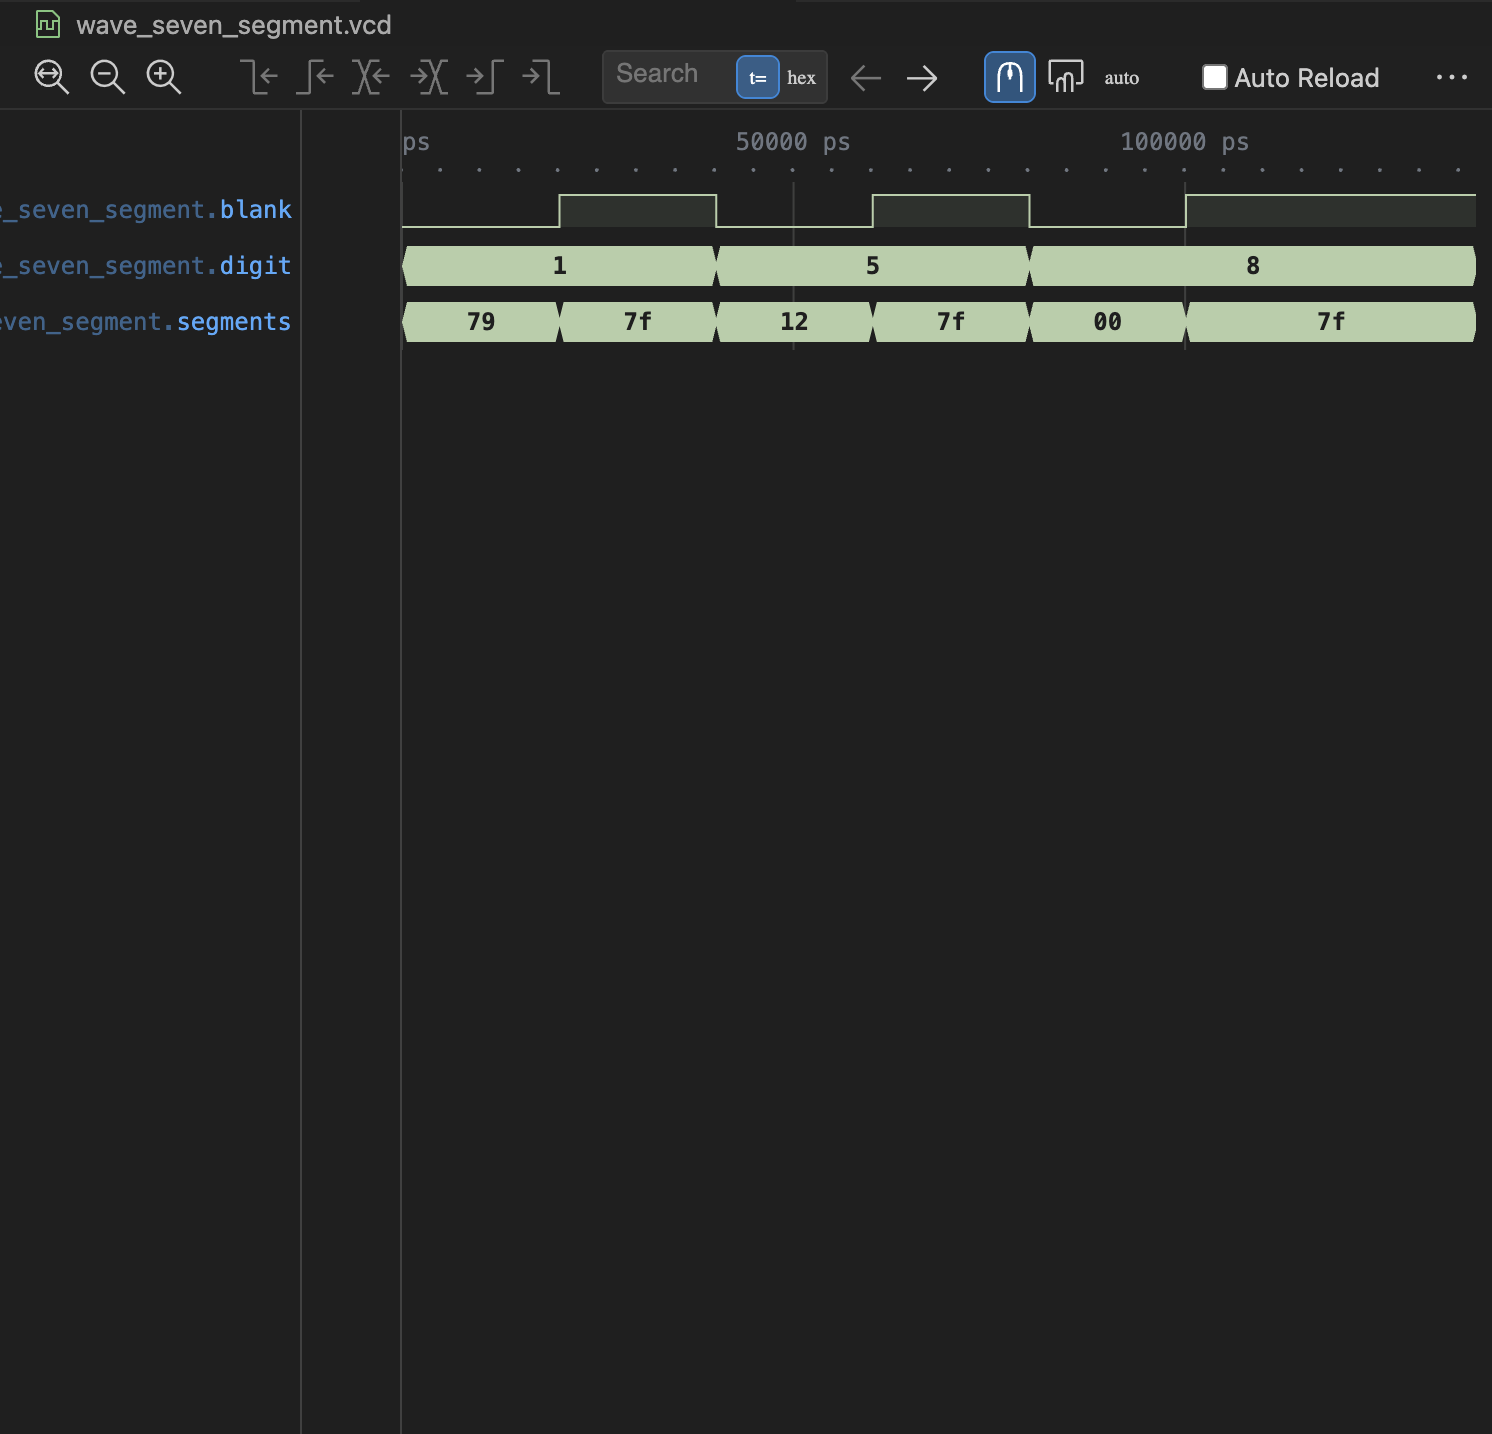
\includegraphics[width=\linewidth]{Images/seven_segment.png}
  \caption{Waveform generated for the seven segment module.}
  \label{fig:ssd}
\end{figure}

\subsection{Module 2: Up Down Counter}
\subsubsection{Waveform}
When the enable signal is low, the counter correctly holds onto the 
current value of 0 (as seen in figure \ref{fig:udc}), before counting up in increments of one when both 
the enable pin and up pin are high. Furthermore, the timer correctly 
counts backwards with a unit of one at the next clock signal after the 
up signal goes low.
\begin{figure}[H]
  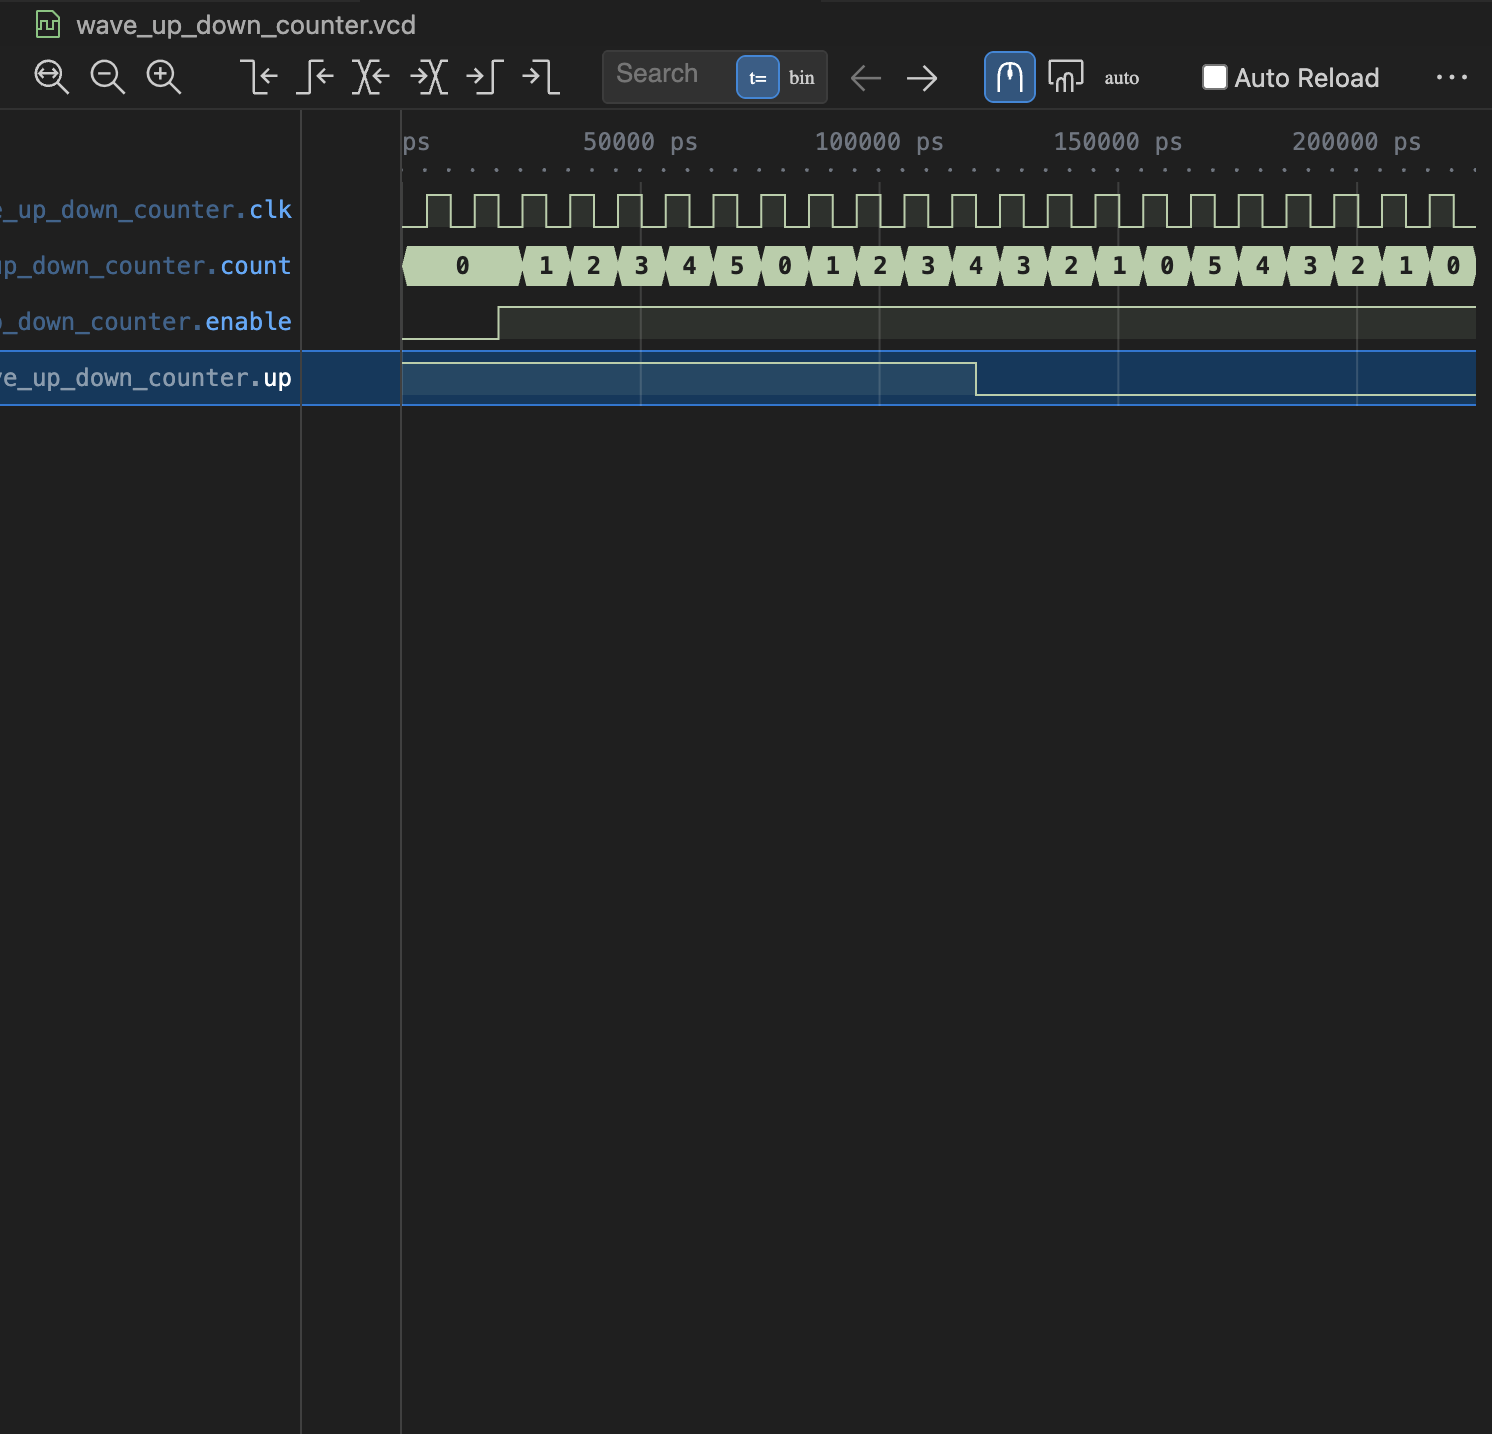
\includegraphics[width=\linewidth]{Images/up_down_counter.png}
  \caption{Waveform generated for the up down counter.}
  \label{fig:udc}
\end{figure}

\subsection{Module 3: Binary to BCD}
\subsubsection{Waveform}
As can be seen with the bin signal of 63 in figure \ref{fig:btb}, the 
circuit correctly breaks down the hexadecimal 63( decimal 99) into the 
ones and tens components of 9 and 9. 
\begin{figure}[H]
  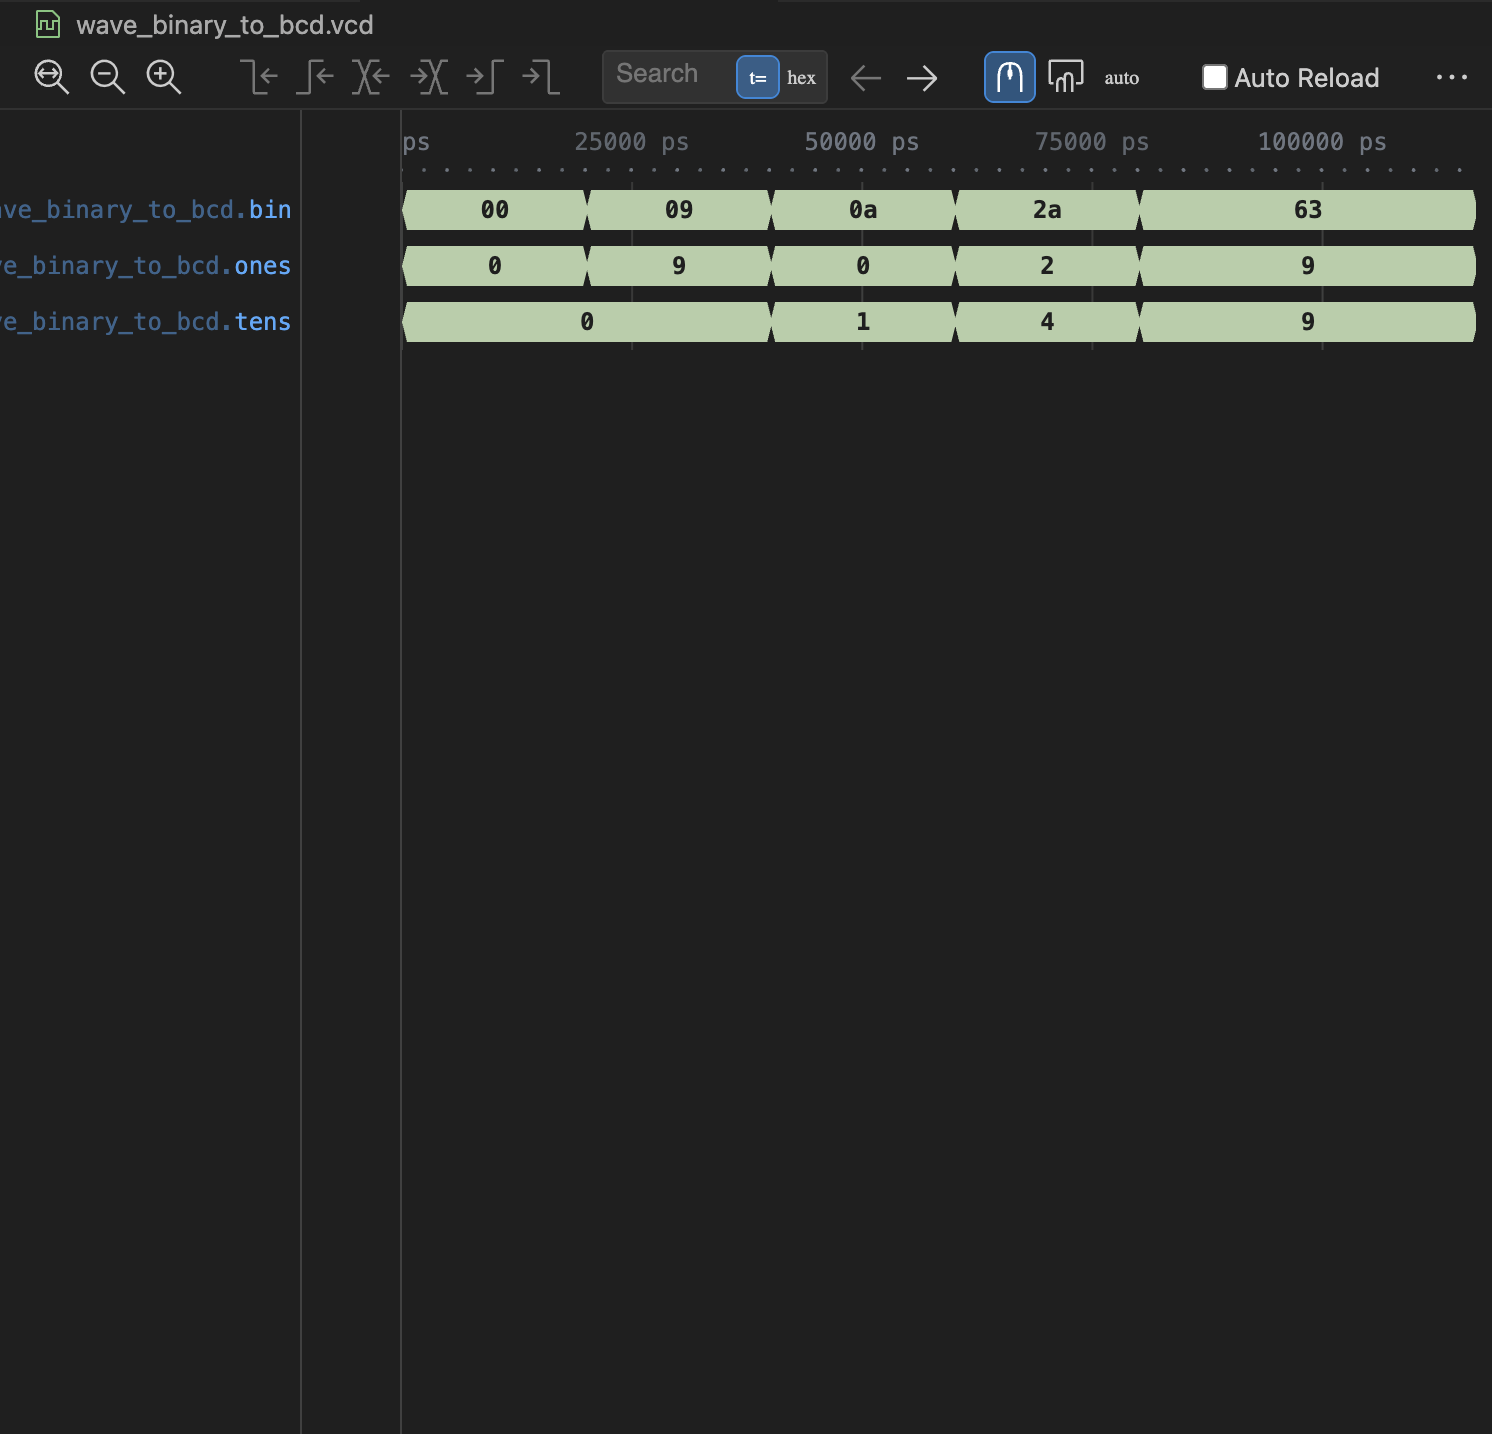
\includegraphics[width=\linewidth]{Images/binary_to_bcd.png}
  \caption{Waveform generated for the binary to bcd converter.}
  \label{fig:btb}
\end{figure}

\subsection{Module 4: HMS Counter}
\subsubsection{Waveform}
The seconds signal of figure /ref{fig:hms} successfully iterates to 4 on
 the rising edge of the rising edge of the clock, where it then switches to 
0 and triggers an iteration in the minutes signal. This is the expected 
 defined bahvaiour given the bit width and max count values used to test 
the circuit. The enable signal is also seen to hold the seconds signal at 0 
from time 0 to the high enable signal.
\begin{figure}[H]
  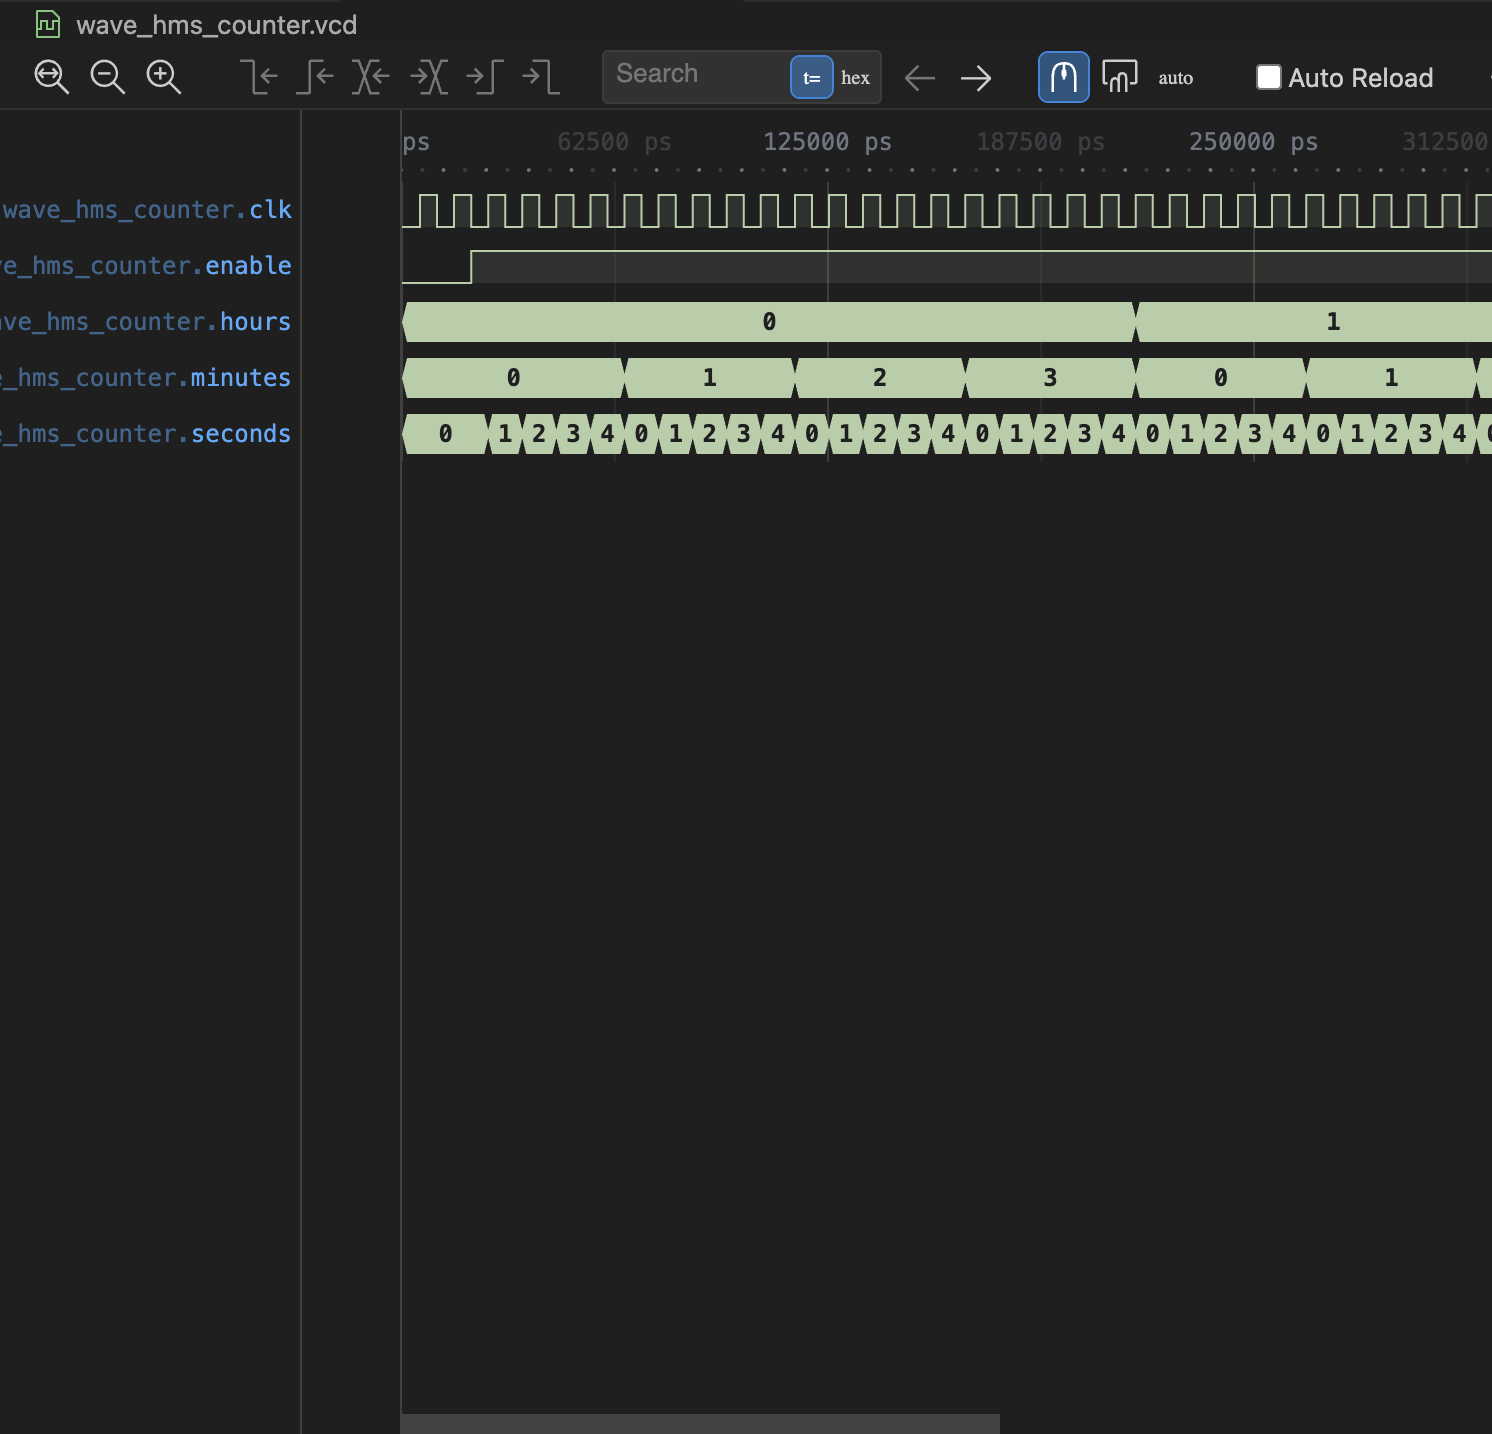
\includegraphics[width=\linewidth]{Images/hms_counter.png}
  \caption{Waveform generated for the HMS counter.}
  \label{fig:hms}
\end{figure}

\subsection{Module 5: Mod N Counter}
\subsubsection{Waveform}
Figure \ref{fig:mnc} demonstrates that the count variable correctly iterates
by one on the rising clock edge only if the enable signal is high and the 
rst signal is low. At the low edge of the rst signal, the counter resets
to 0 at the next rising edge of the clock. At the low edge of the enable 
signal the counter holds its previous value.
\begin{figure}[H]
  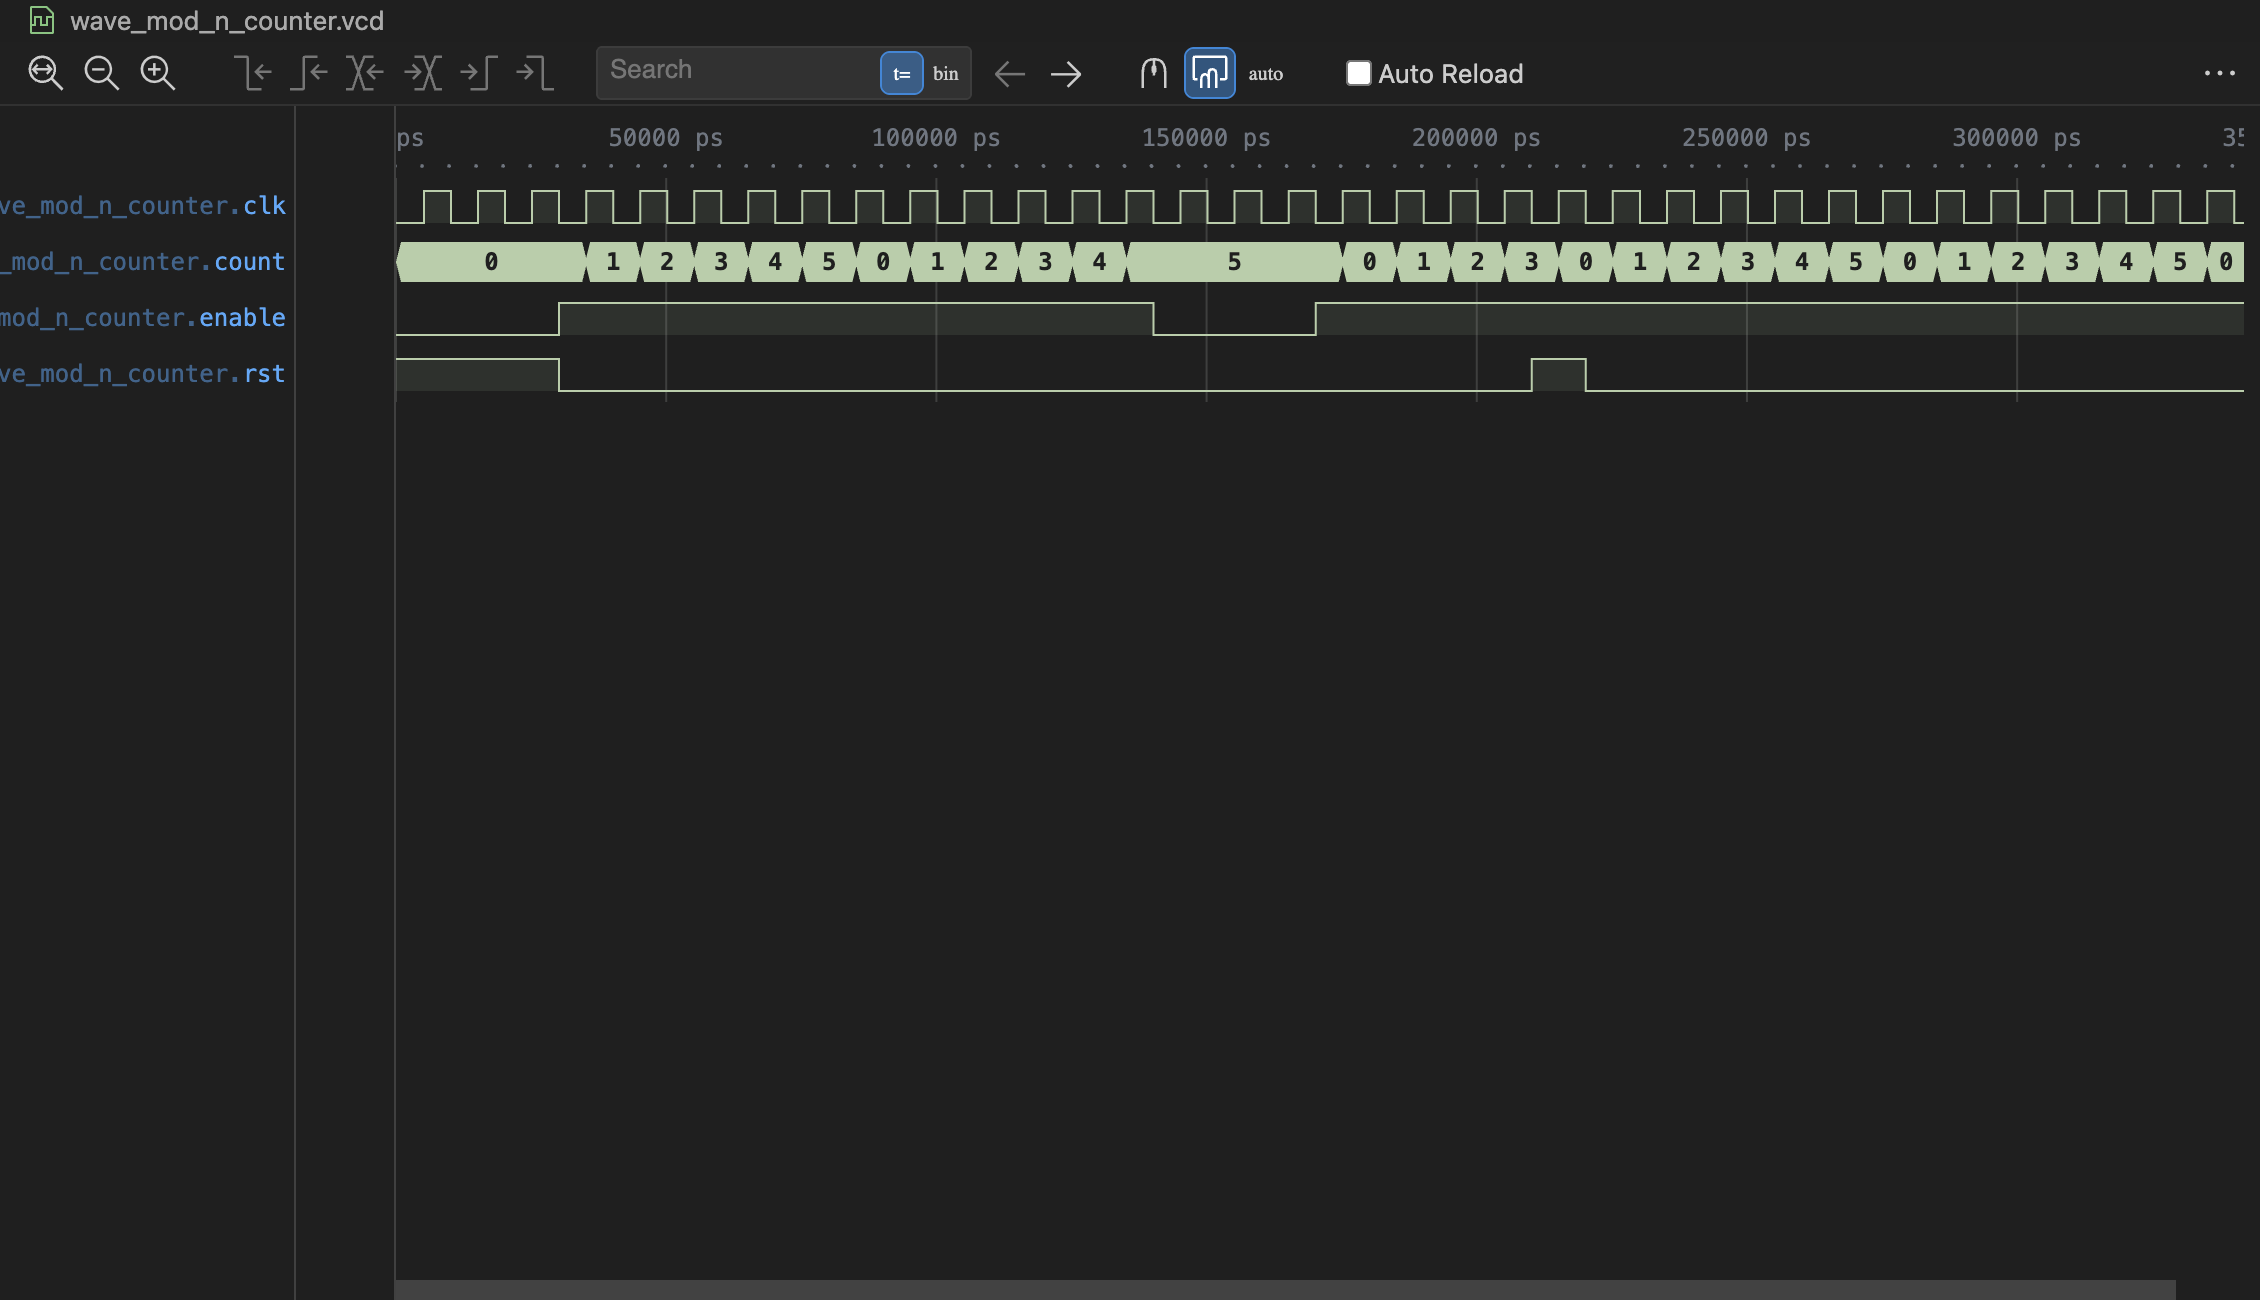
\includegraphics[width=\linewidth]{Images/mod_n_counter.png}
  \caption{Waveform generated for the mod n counter.}
  \label{fig:mnc}
\end{figure}

\subsection{Module 6: Restartable Rate Generator}
\subsubsection{Waveform}
Figure \ref{fig:rrg} shows that the tick signal will pulse for one
clock cycle when the counter reaches it's maximum value defined by 
CYCLE\_COUNT. The running signal correctly follows the run signal 
with a clock cycle delay. Furthermore, the counter resets each clock 
cycle that the running signal is low.
\begin{figure}[H]
  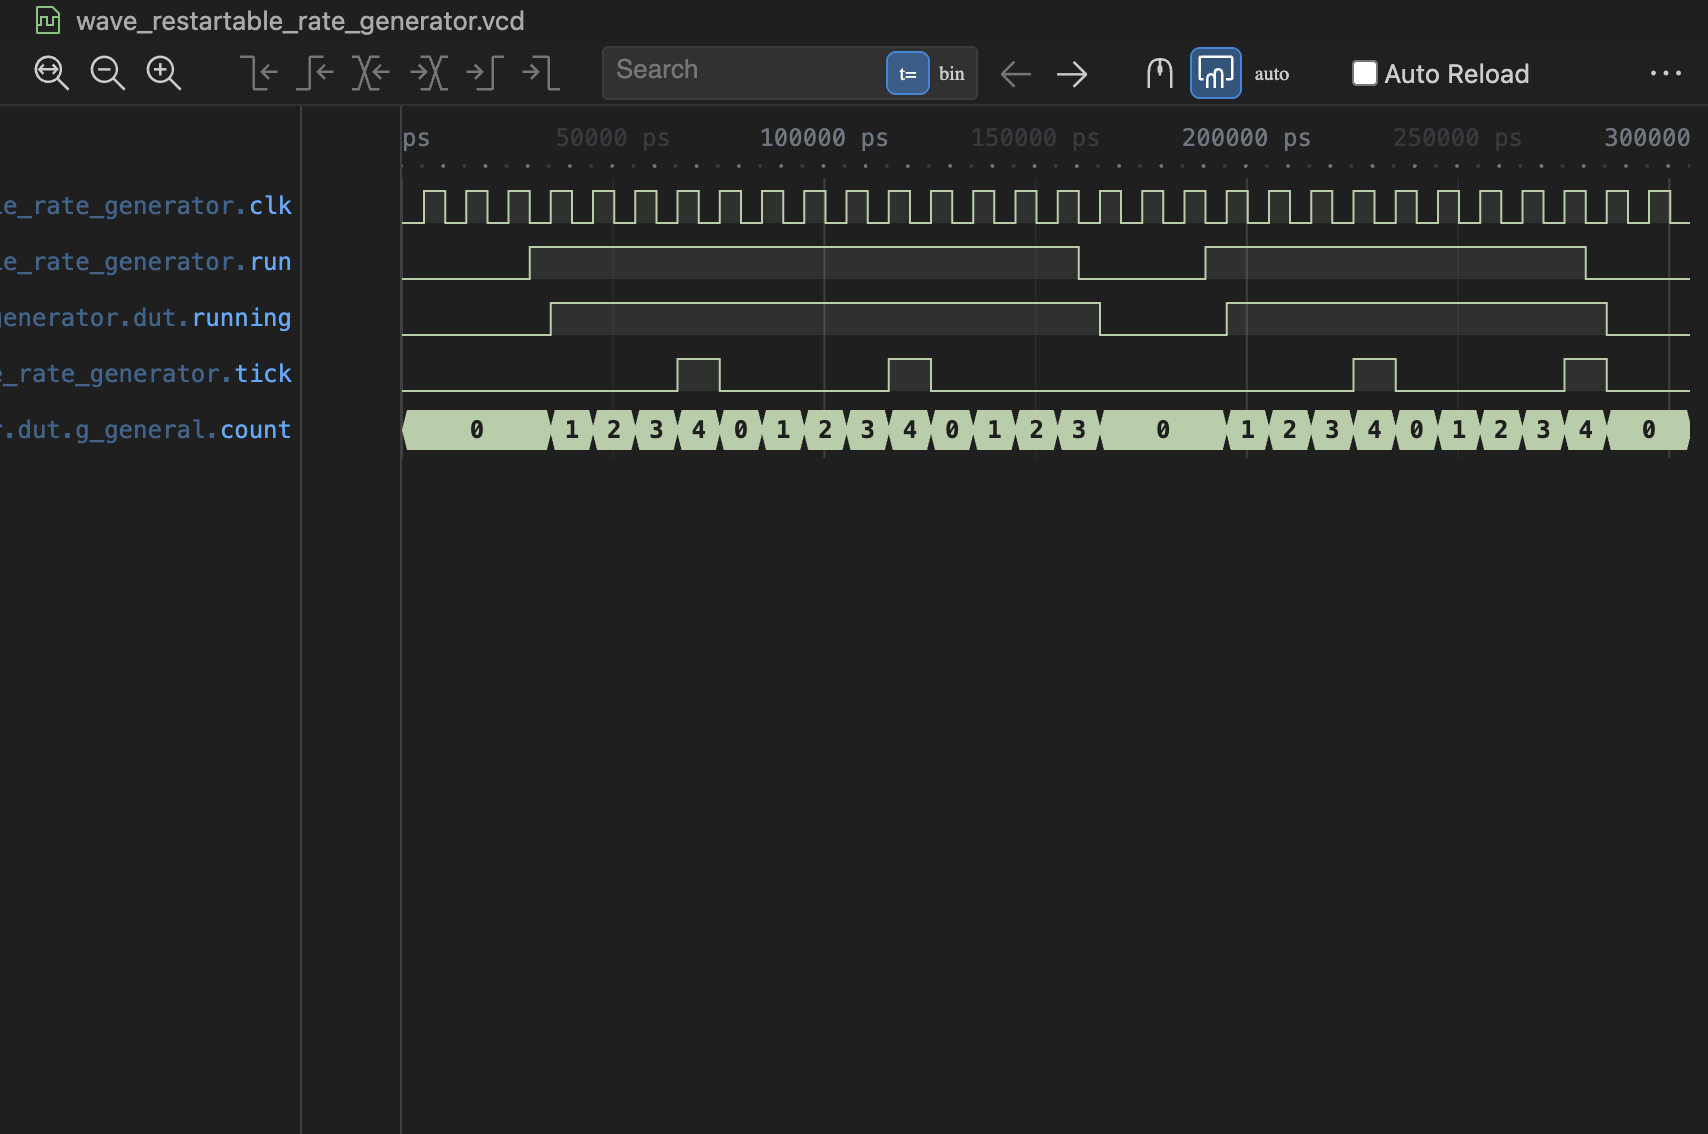
\includegraphics[width=\linewidth]{Images/restartable_rate_generator.png}
  \caption{Waveform generated for restartable rate generator.}
  \label{fig:rrg}
\end{figure}

\subsection{Module 7: Top Time Display (v1)}
\subsubsection{Waveform}
Figure \ref{fig:ttdv1} demonstrates a initial pause as the input switch 
specifies the longest second period. After the timer is switched to the 
faster clock mode, the seconds correct increments by one with the hexadecimal 
output directly matching the seconds input. The seconds count reaches 59 
and rolls over, incrementing the minute count by 1 which is mirrored in the 
hexadecimal output signal. This behaviour continues through the test.
\begin{figure}[H]
  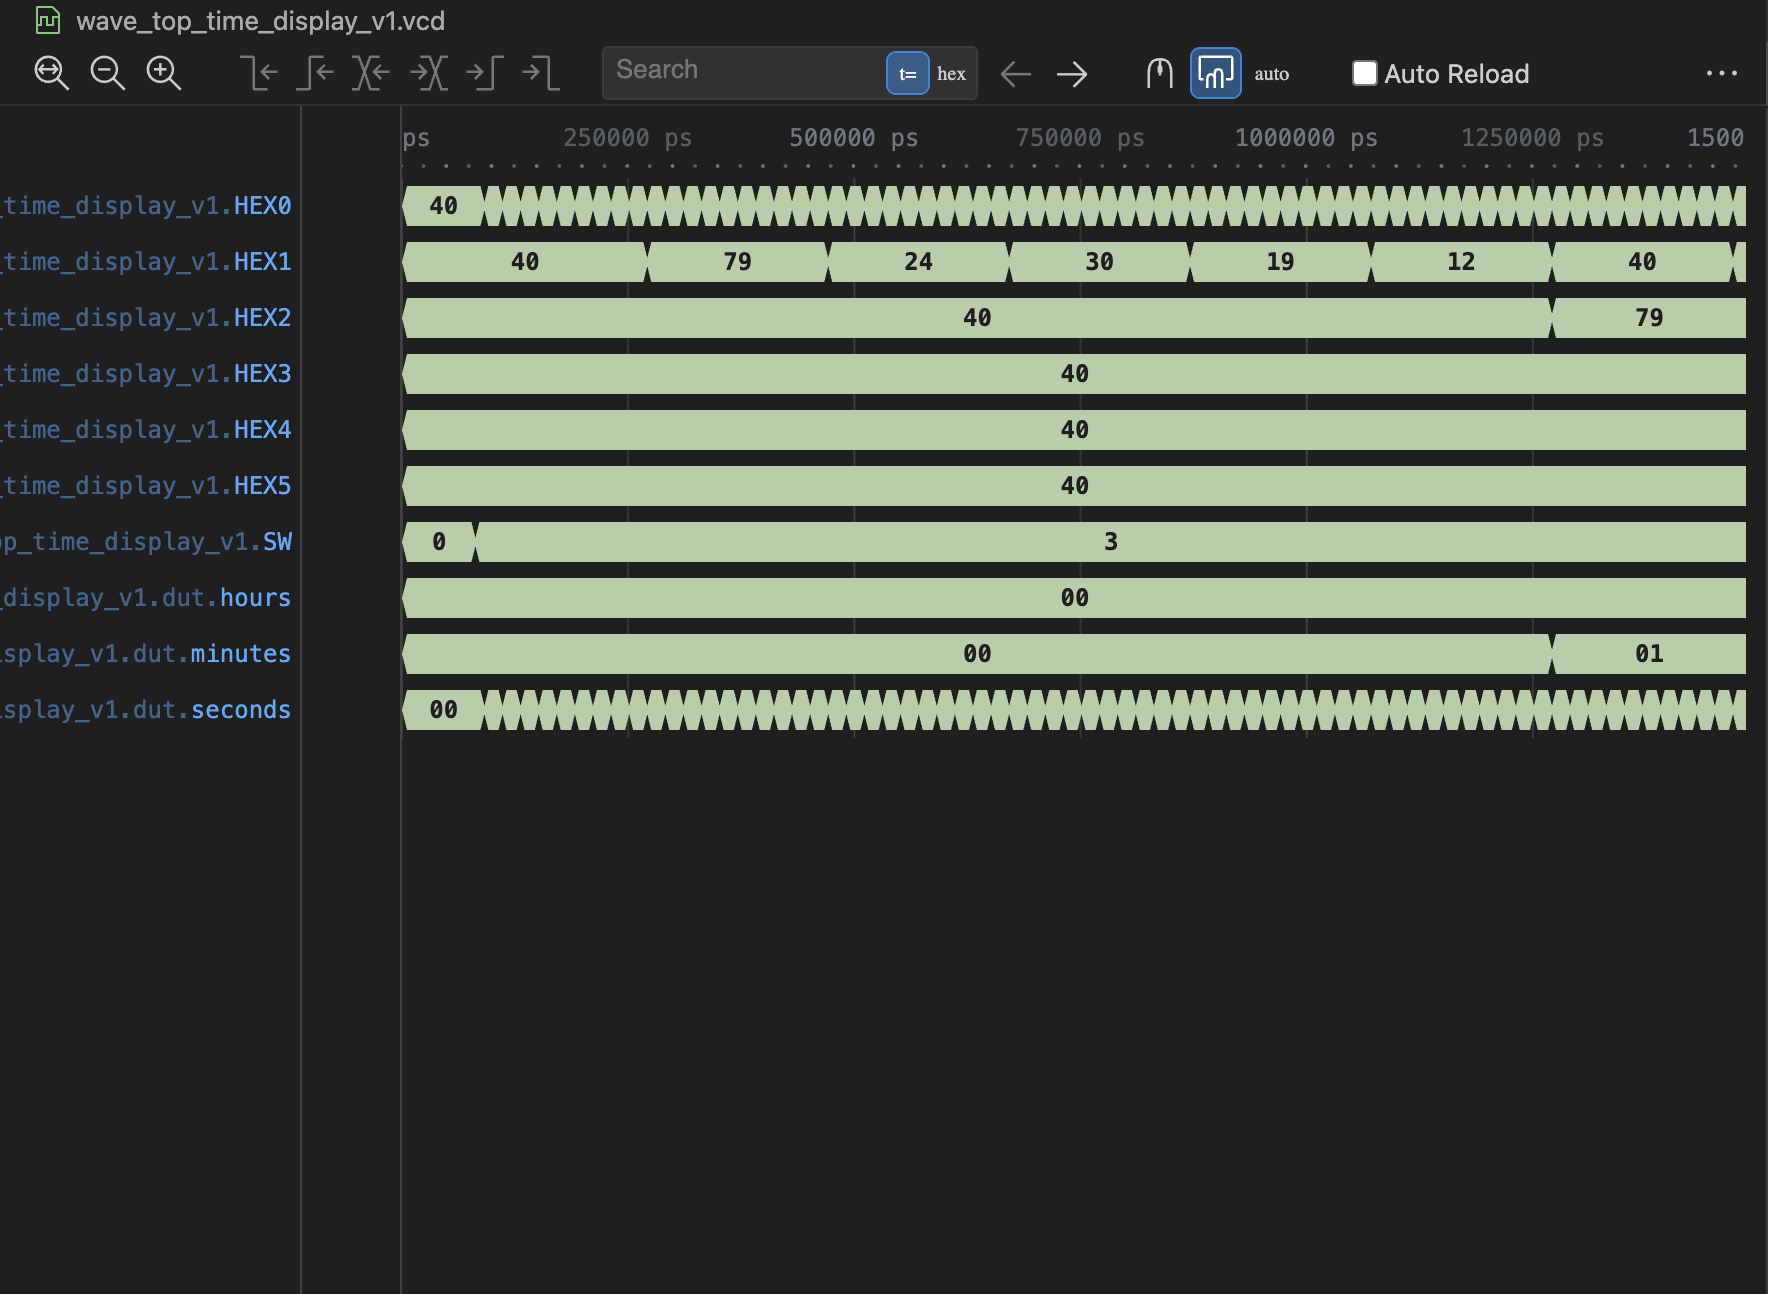
\includegraphics[width=\linewidth]{Images/top_time_display_v1.png}
  \caption{Waveform generated for the first top time display.}
  \label{fig:ttdv1}
\end{figure}

\subsection{Module 8: Pulse Width Modulation Generator}
\subsubsection{Waveform}
Figure \ref{fig:pwm} shows that the count signal increments
to the cycle number, and correctly holds at 0 when the rst signal is 
high. The PWM signal holds at 1 for the specified duty cycle, and
remains at 0 for the rest of the period.
\begin{figure}[H]
  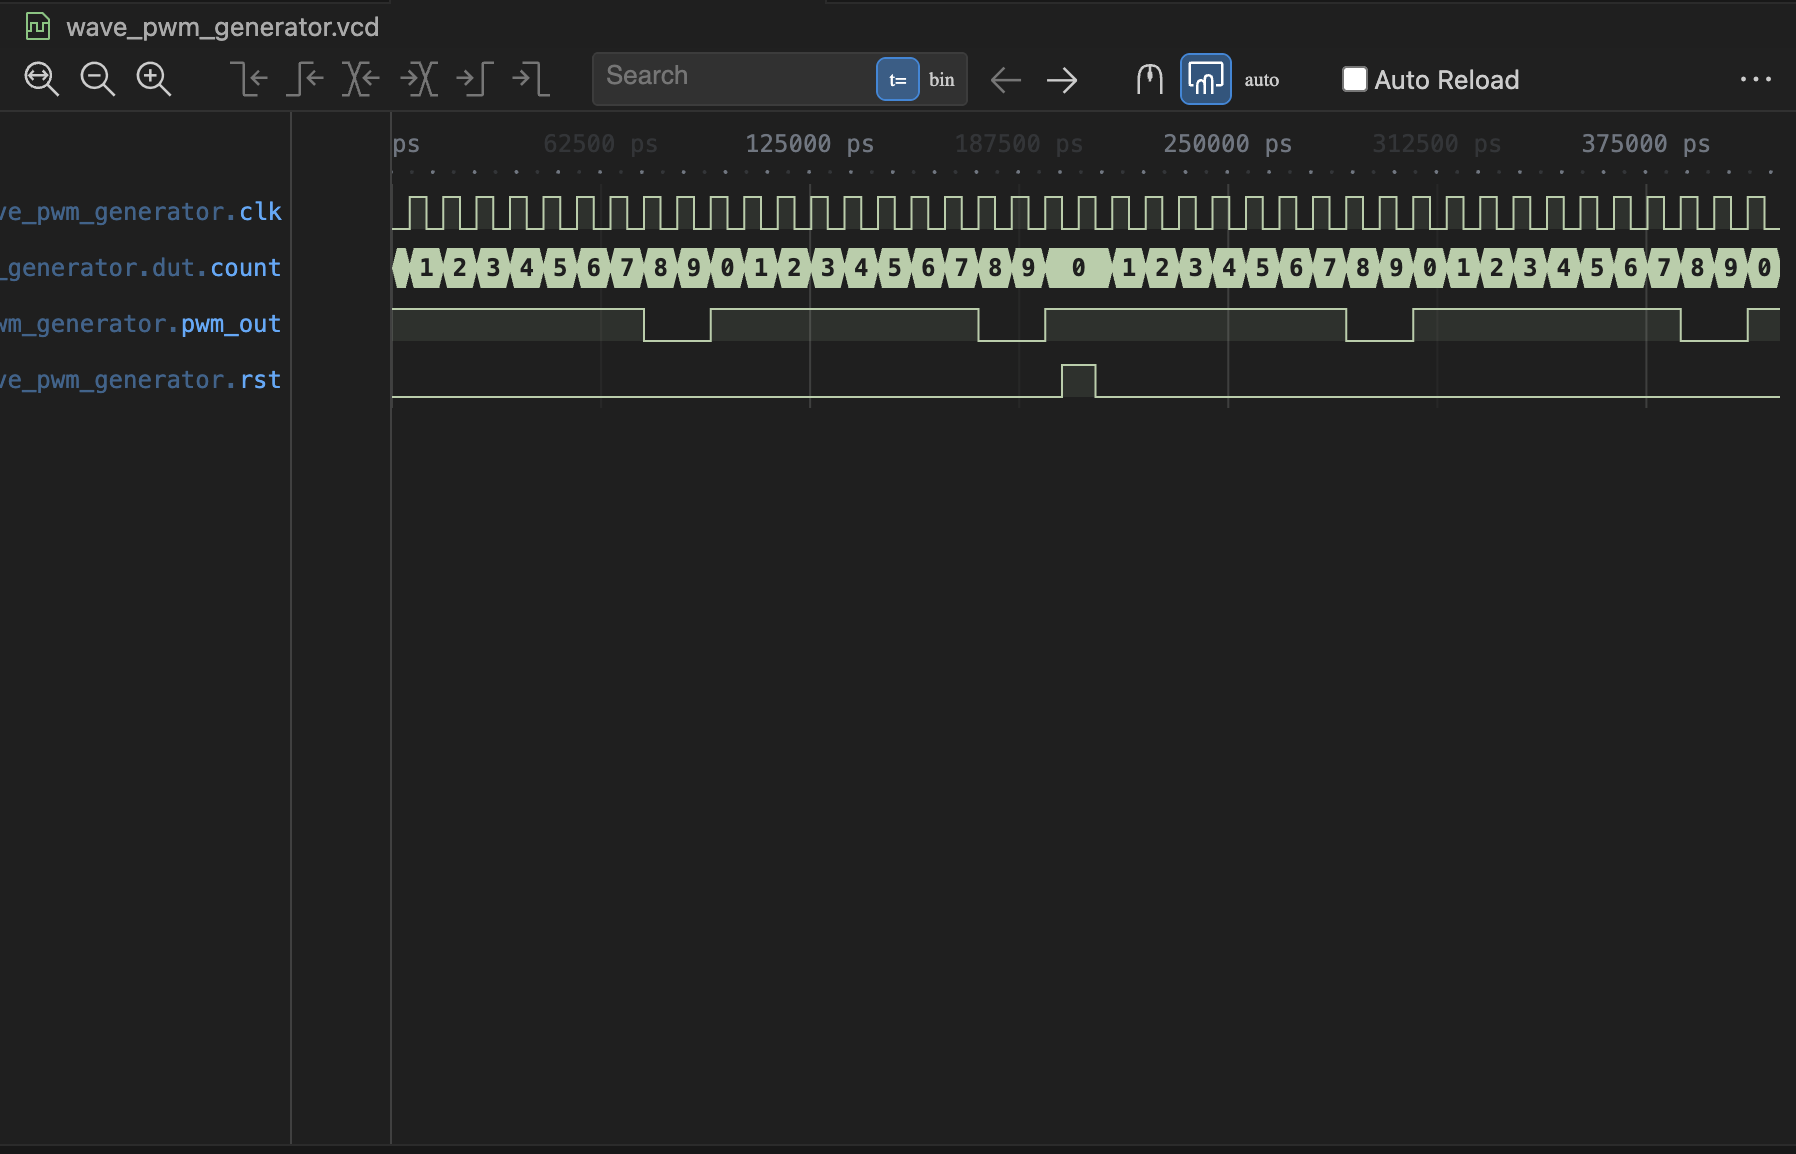
\includegraphics[width=\linewidth]{Images/pwm_generator.png}
  \caption{Waveform generated for pwm generator.}
  \label{fig:pwm}
\end{figure}

\subsection{Module 9: Rising Edge Detector}
\subsubsection{Waveform}
Figure \ref{fig:red} demonstrates a clock cycle wide pulse on the 
pwm\_out signal when the sig\_in signal goes high and the clock pulses. 
If the pulse occurs within a clock cycle, no output occurs as expected.
\begin{figure}[H]
  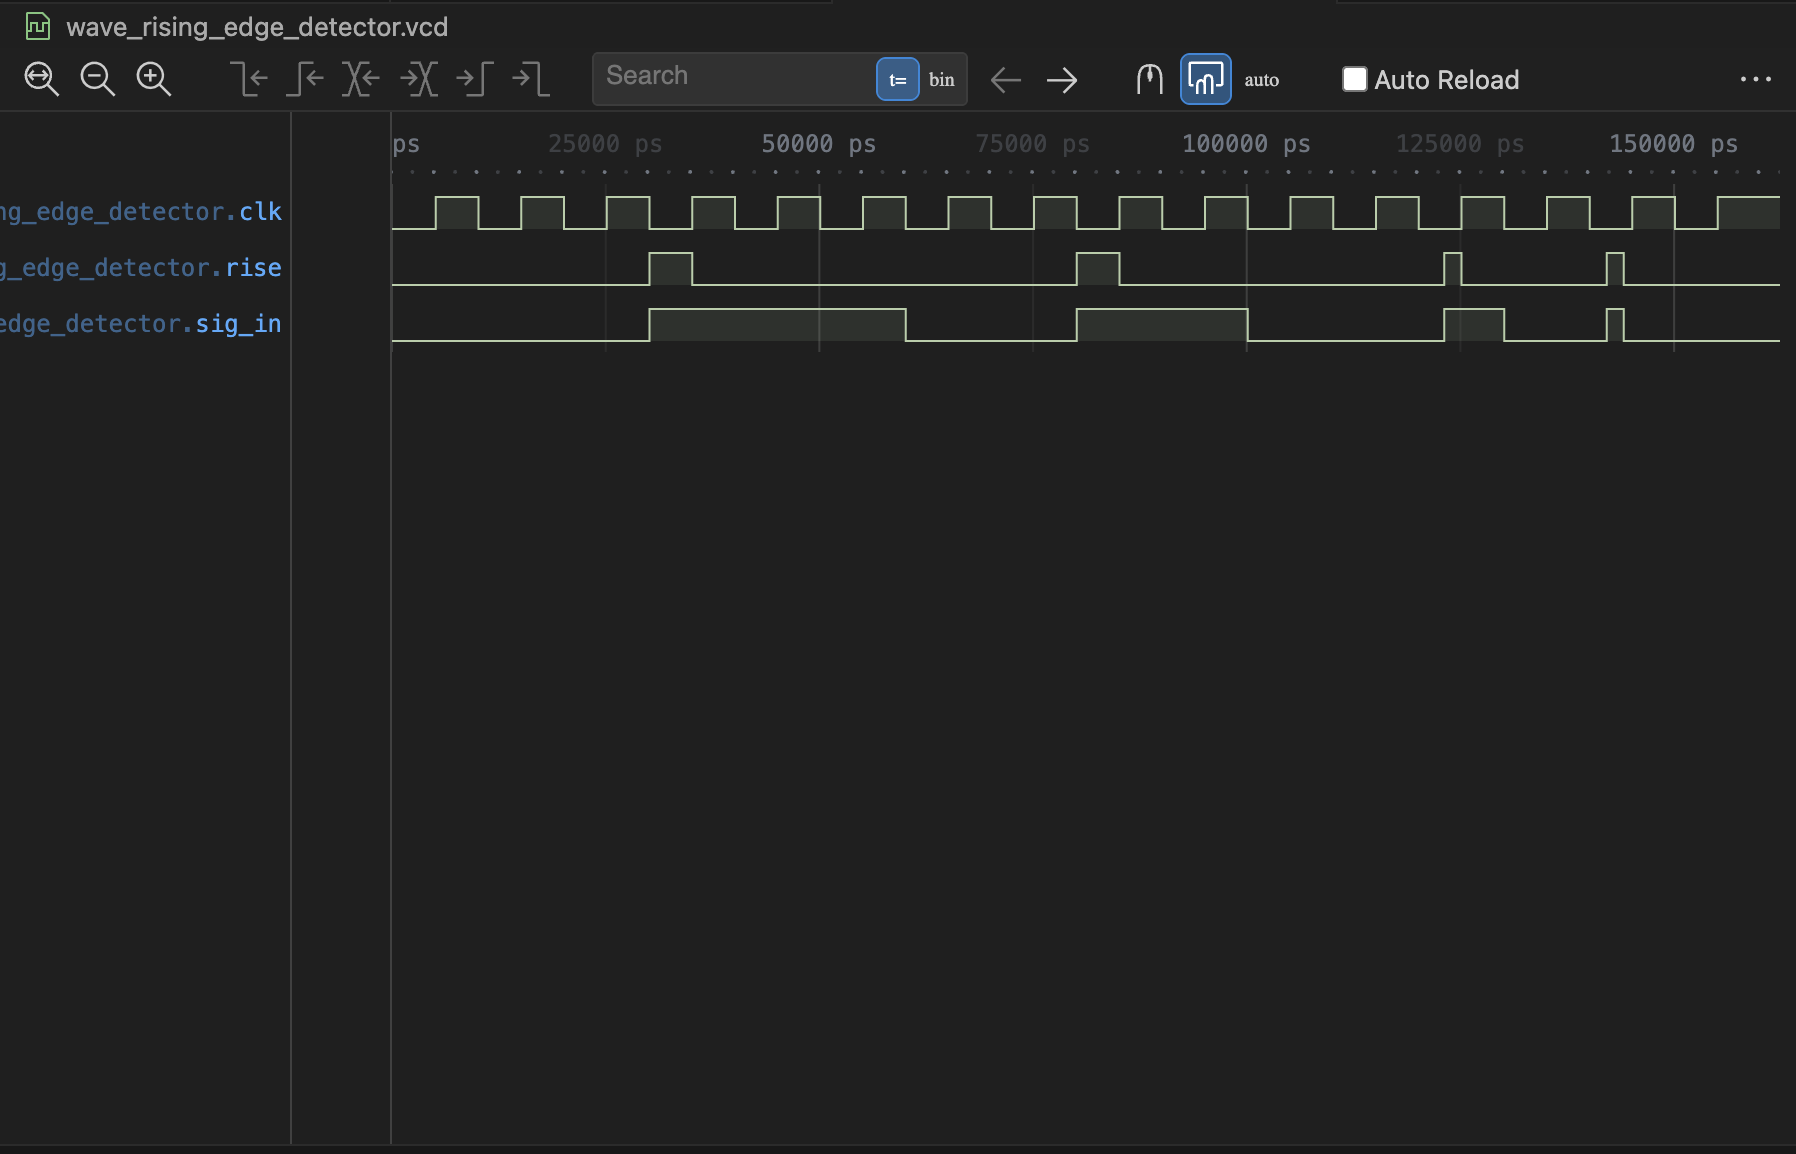
\includegraphics[width=\linewidth]{Images/rising_edge_detector.png}
  \caption{Waveform generated for rising edge detector.}
  \label{fig:red}
\end{figure}

\subsection{Module 10: Button Hold Detect}
\subsubsection{Waveform}
Figure \ref{fig:bhd} shows that the counter resets every cycle untill
the button is pressed, for which it begins to count at the next clock cycle 
while the button remains pressed. If the counter reaches the specified 
number of cycles, the held signal will go high. This disables the counter 
and holds the held signal high untill the button is released and the 
counter is reset. 
\begin{figure}[H]
  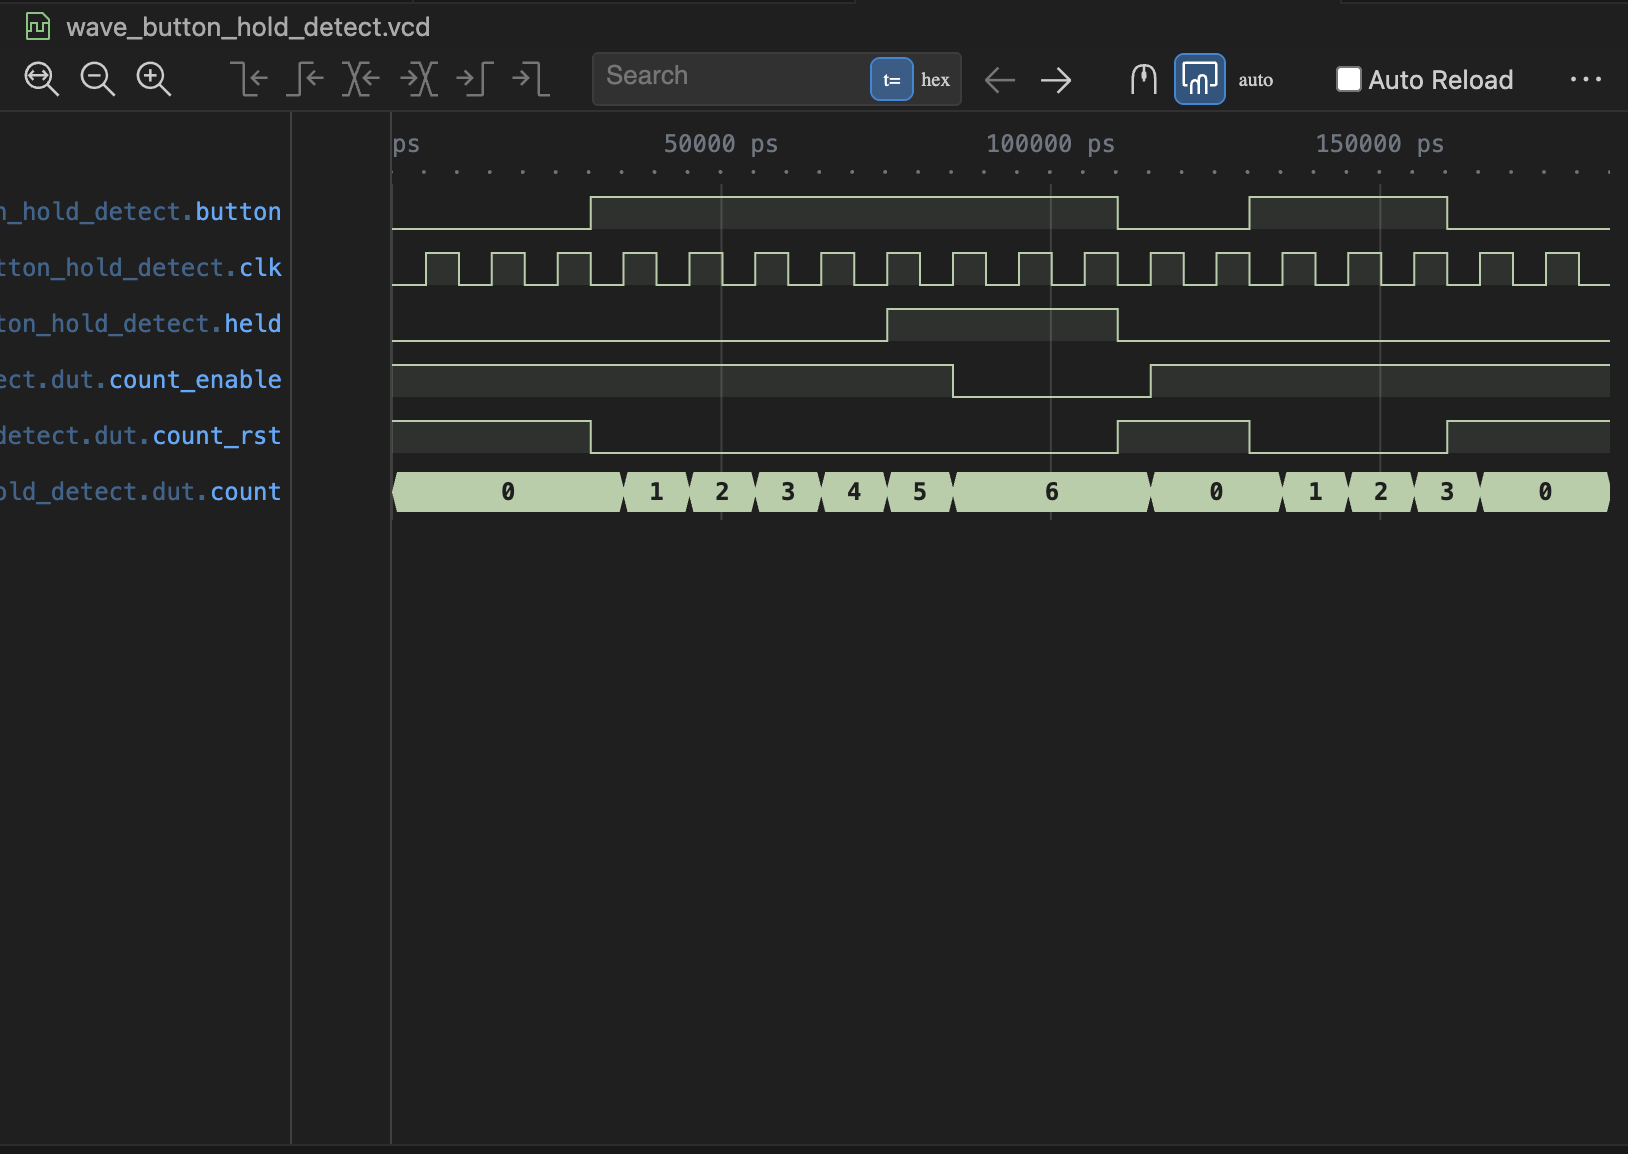
\includegraphics[width=\linewidth]{Images/button_hold_detect.png}
  \caption{Waveform generated for the button hold detector.}
  \label{fig:bhd}
\end{figure}

\subsection{Module 11: Button Hold Pulse}
\subsubsection{Waveform}
Figure \ref{fig:bhp} shows a pulse signal one clock cycle wide triggered
only after the button signal has been held high for a specified number of 
clock cycles. No pulse occurs if the button is not held down for the specified 
number of clock cycles, and the pulse signal does not remain high as the 
previous module specified.
\begin{figure}[H]
  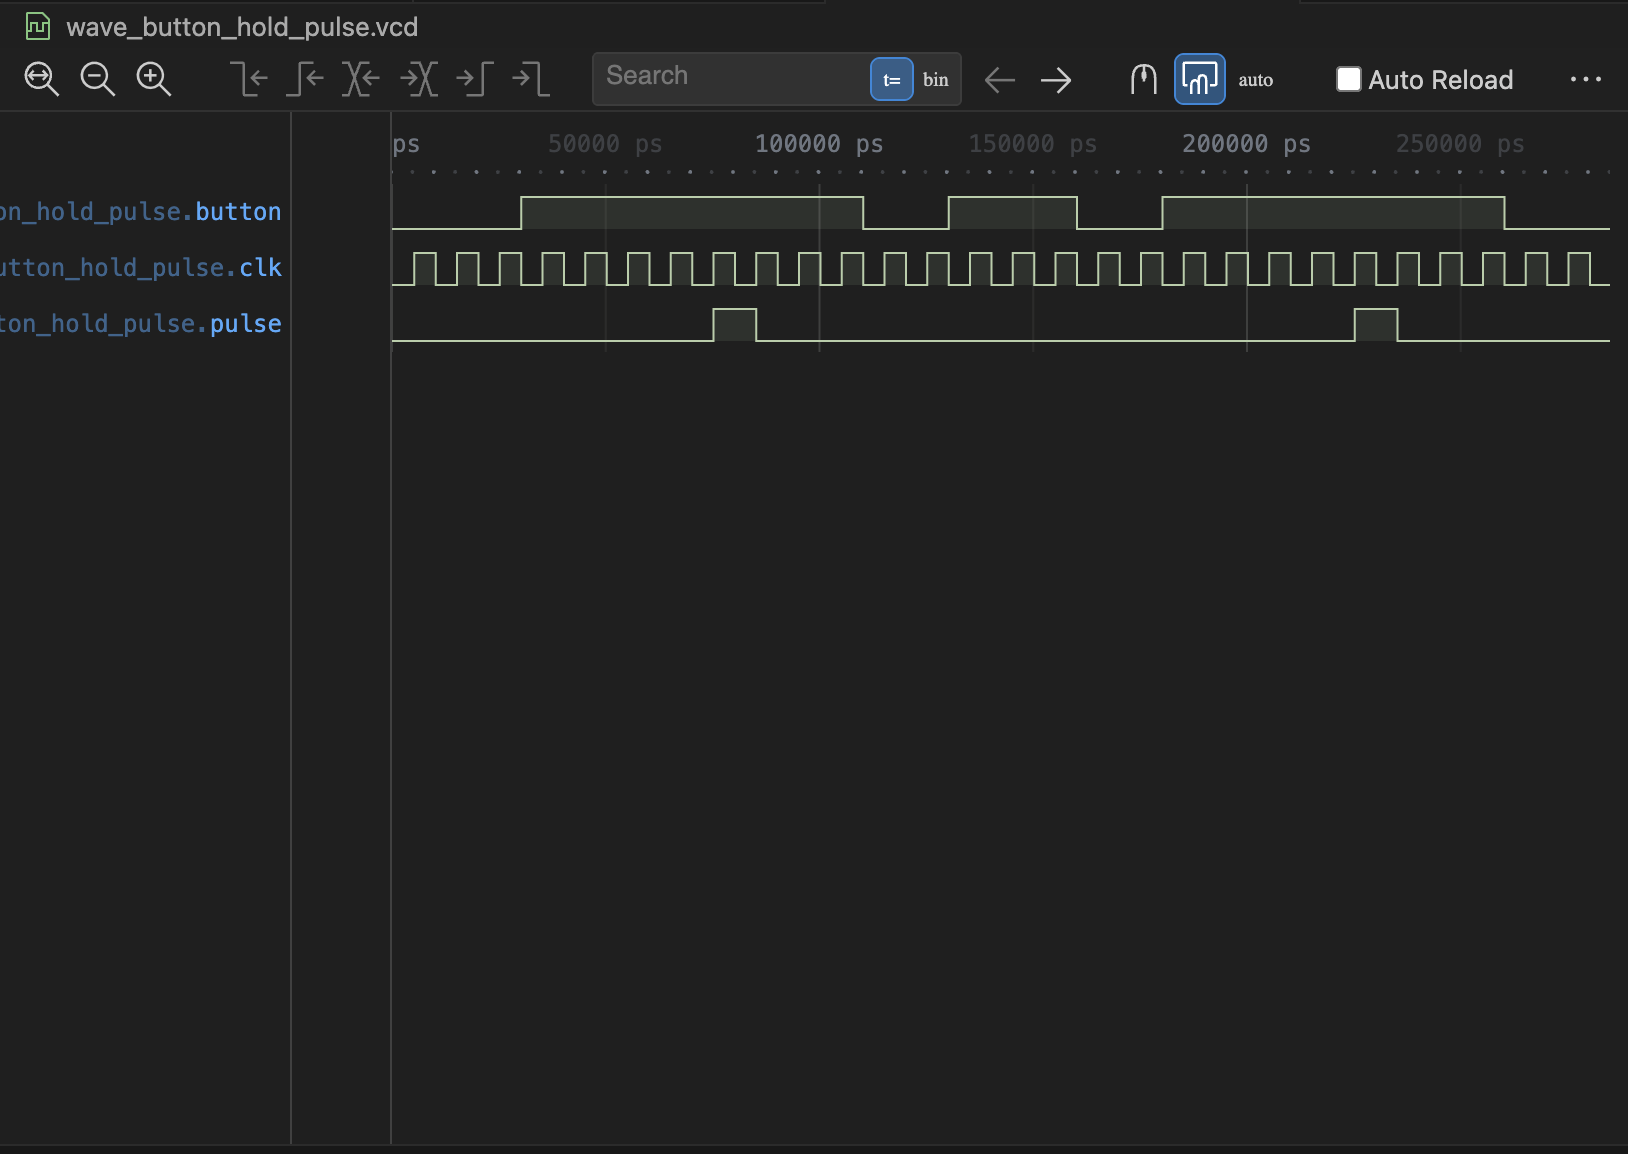
\includegraphics[width=\linewidth]{Images/button_hold_pulse.png}
  \caption{Waveform generated for the button hold pulser.}
  \label{fig:bhp}
\end{figure}

\subsection{Module 12: Button Auto Repeat}
\subsubsection{Waveform}
The pulse signal in figure \ref{fig:bar} demonstrates a breif pulse 
cuttoff by the next clock rising edge as the button signal goes high. 
The counter then begins in the button\_hold\_detect module which produces 
a high signal after 7 clock pulses which feeds the run signal of the 
rate generator. The rate generator produces a periodic pulse on the pulse 
wire until the button is released.
\begin{figure}[H]
  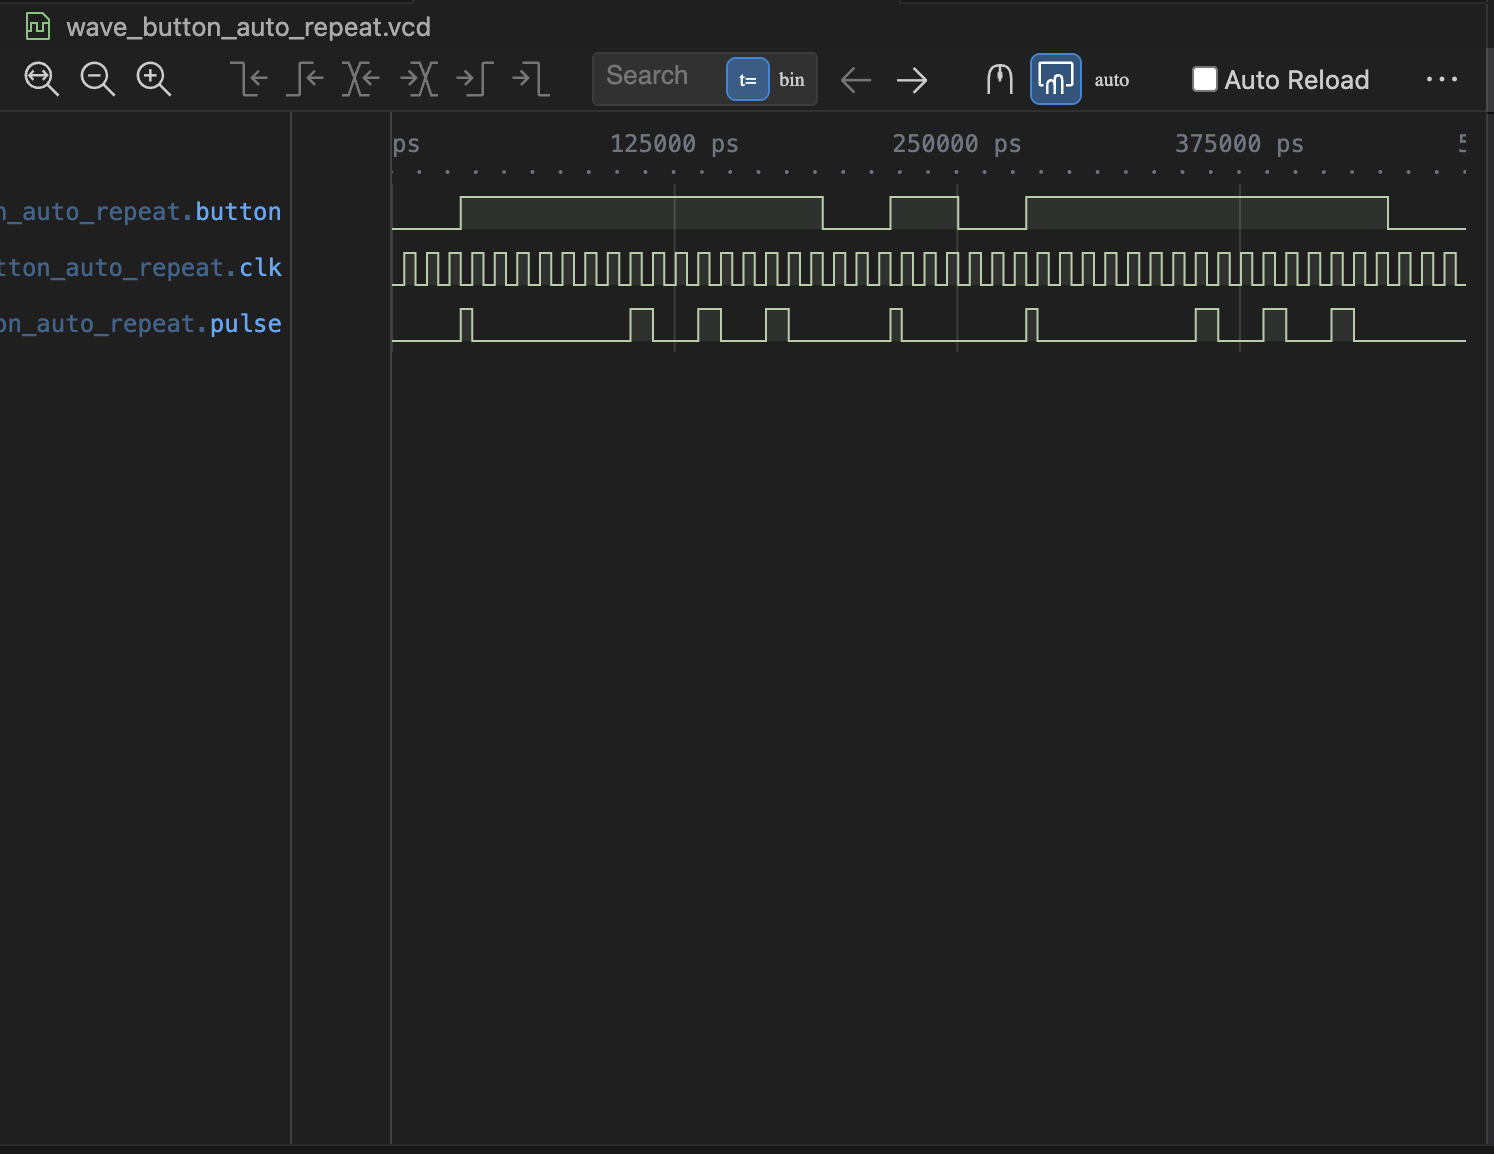
\includegraphics[width=\linewidth]{Images/button_auto_repeat.png}
  \caption{Waveform generated for the button auto repeat module.}
  \label{fig:bar}
\end{figure}

\subsection{Module 13: Arming Latch}
\subsubsection{Waveform}
The armed signal in figure \ref{fig:alr} goes high at the next clock cycle 
after the arm signal has gone high, and the disarm signal is low. The 
armed signal stays high untill the disarm signal is pulled high. If 
both the arm and disarm signals go high, the disarm signal takes 
priority.
\begin{figure}[H]
  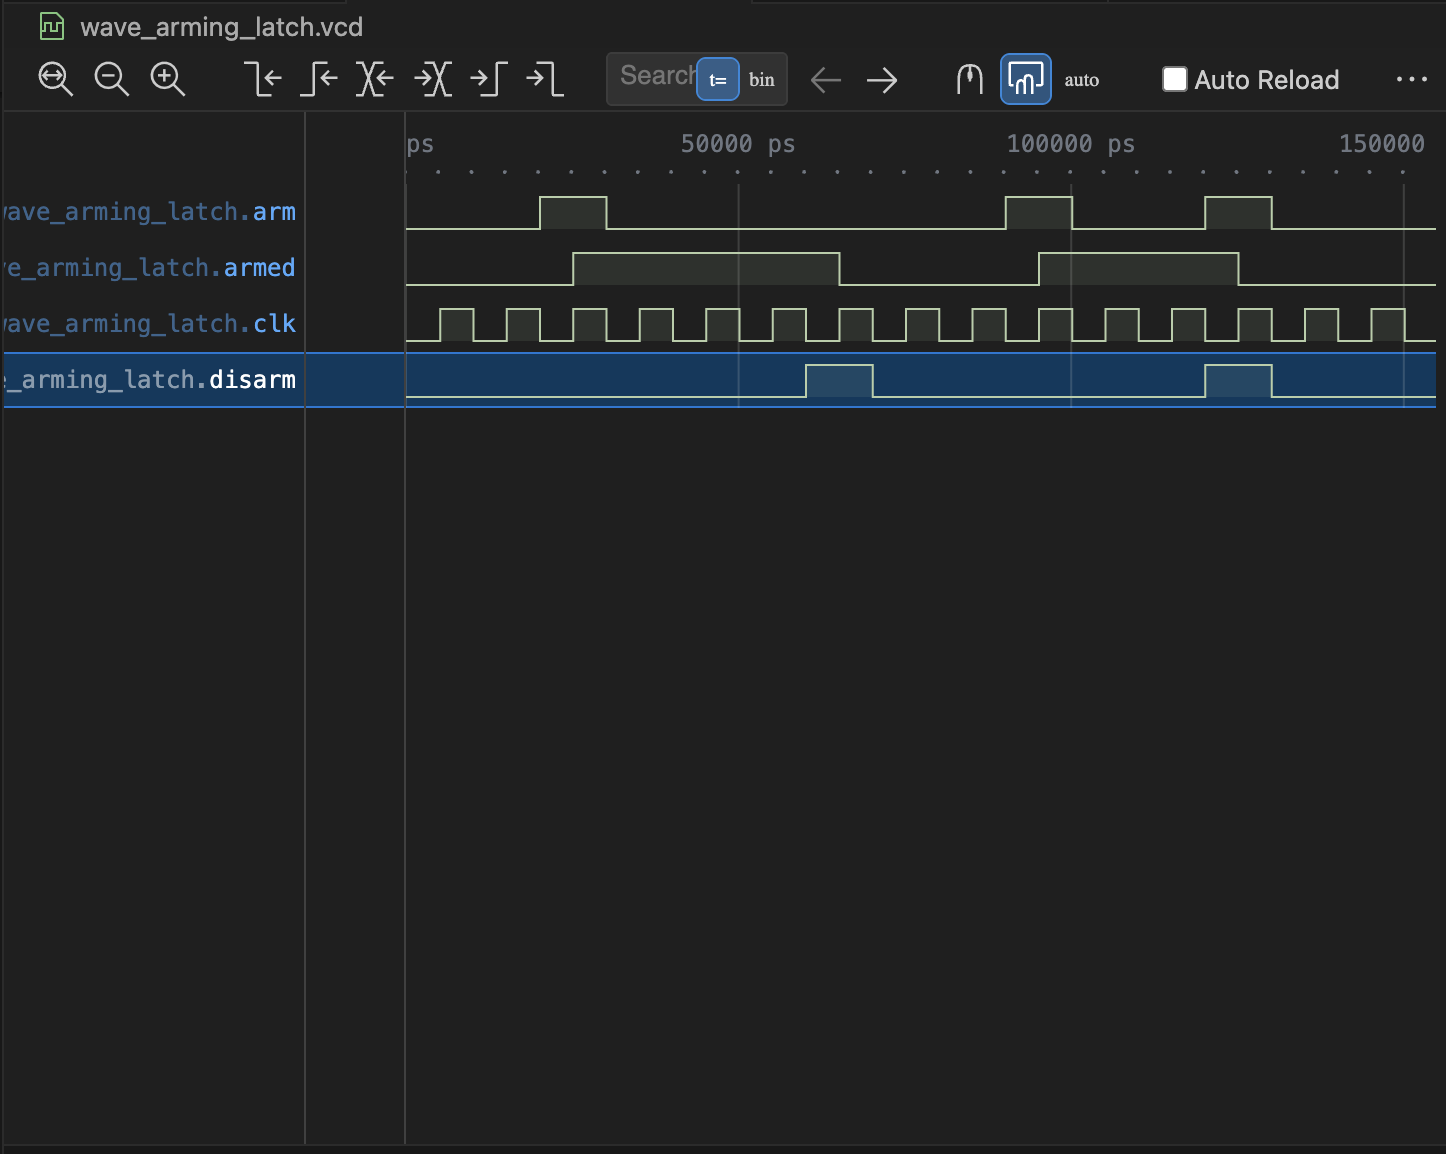
\includegraphics[width=\linewidth]{Images/armed_latch.png}
  \caption{Waveform generated for the armed latch.}
  \label{fig:al}
\end{figure}

\subsection{Module 14: Edit Mode Selector}
\subsubsection{Waveform}
Figure \ref{fig:ems} demonstrates that the button must remain pressed 
for the specified number of clock cycles to enter seconds mode. Later 
breif presses shift the state into minutes mode, and then hours mode 
before reseting the counter and disarming the system.
\begin{figure}[H]
  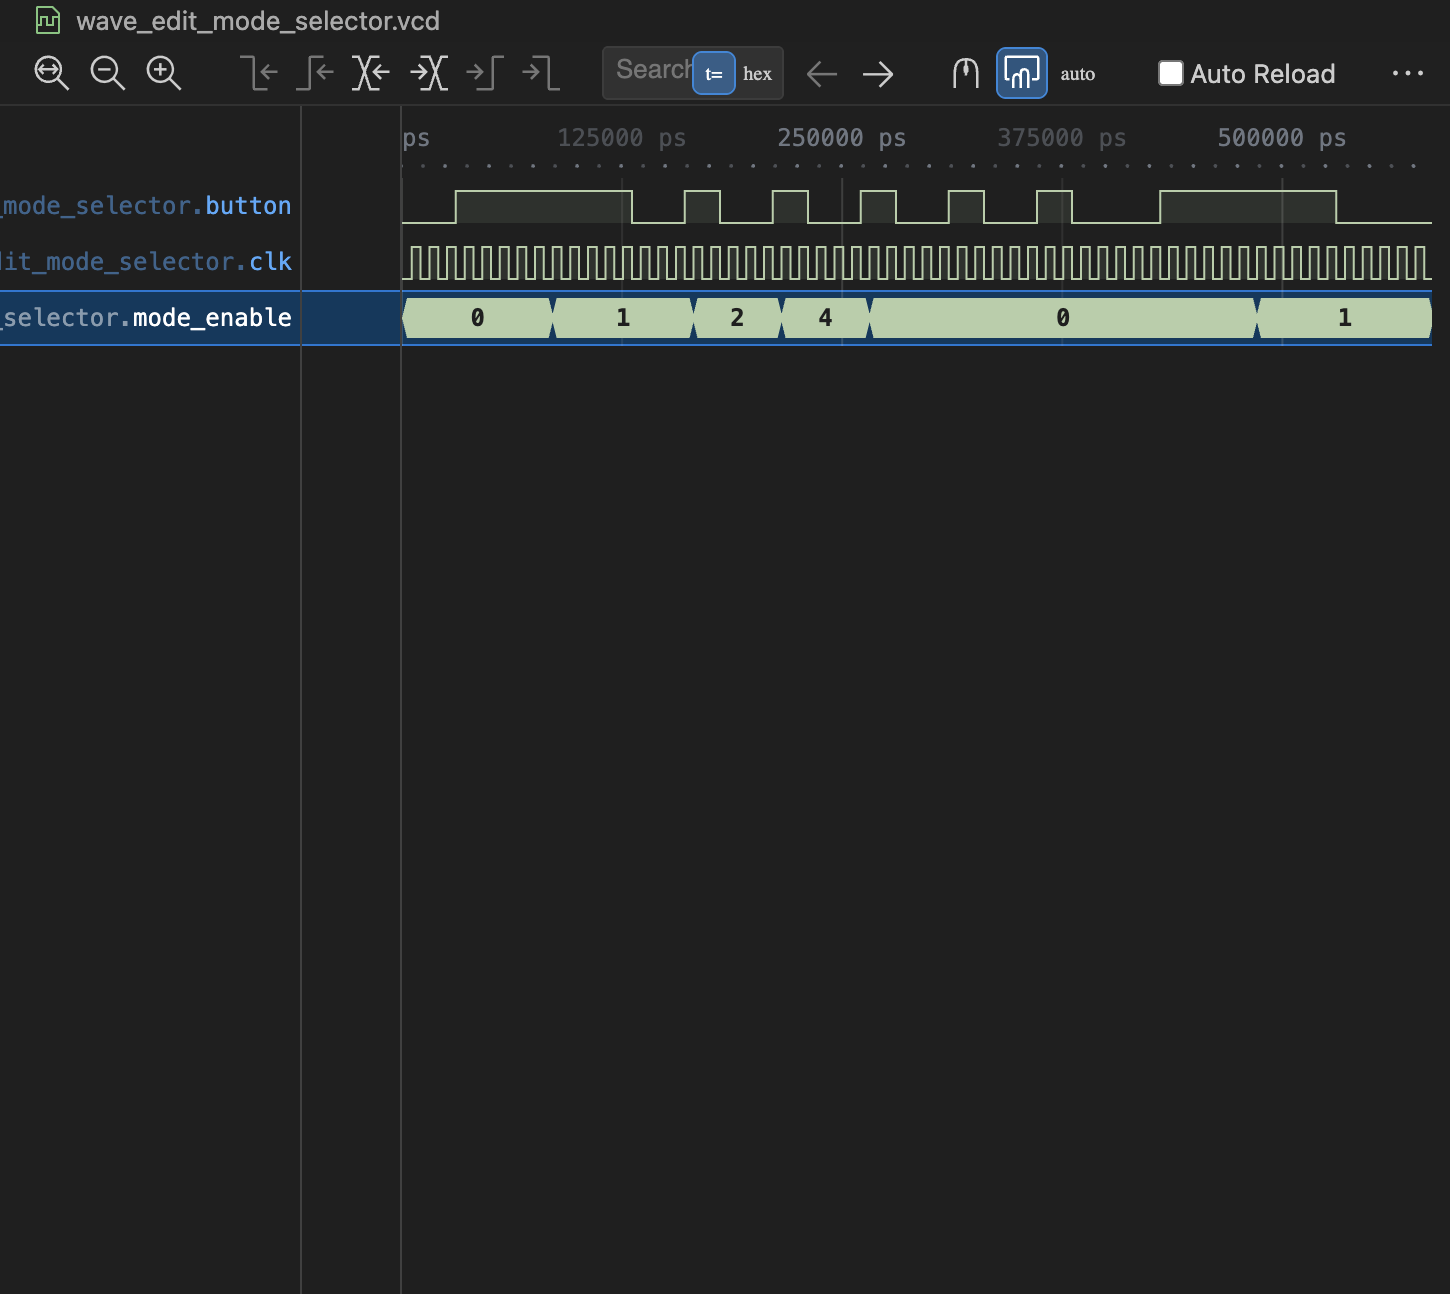
\includegraphics[width=\linewidth]{Images/edit_mode_selector.png}
  \caption{Waveform generated for the edit mode selector module.}
  \label{fig:ems}
\end{figure}

\subsection{Module 15: Editable Counter}
\subsubsection{Waveform}
The counter increments with tick when edit mode is off as seen in 
Figure \ref{fig:ec}. Once the edit mode signal is pulled high, the 
inc signal is pulled high which initially increments the counter, before 
the tick signal continues to increment the counter. When dec mode is enabled, 
the counter conitnually counts down before wrapping around to the maximum 
value. When both the inc and dec signals are high, the counter does 
nothing. Once the edit mode signal goes low, the counter continues to 
increment with the tick signal.
\begin{figure}[H]
  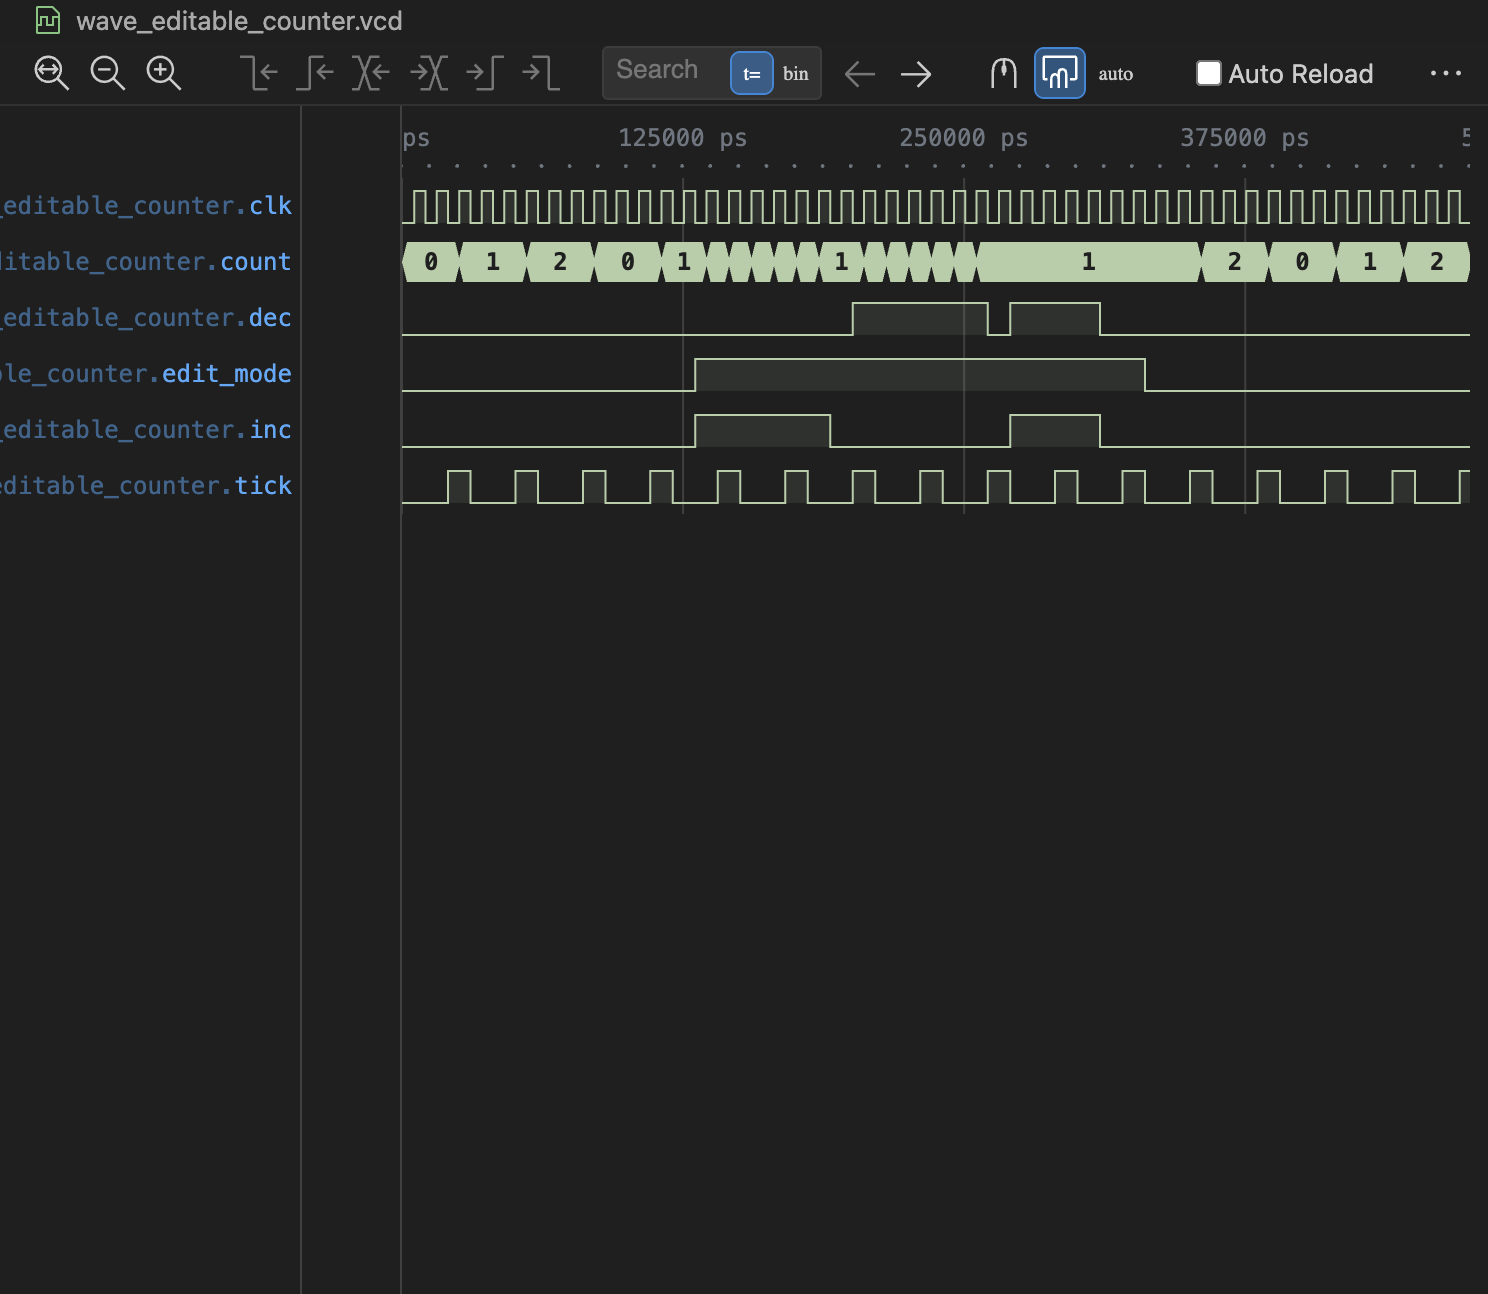
\includegraphics[width=\linewidth]{Images/editable_counter.png}
  \caption{Waveform generated for the editable counter.}
  \label{fig:ec}
\end{figure}

\subsection{Module 16: Key Synchroniser}
\subsubsection{Waveform}
The key state is inverted and stored in the key register at the next clock 
rising edge as seen in figure \ref{fig:ks}. On the next rising edge 
the inverted key state is transfered to the key\_sync\_next register 
which is directly linked to the key\_ sync output. The waveform also 
demonstrates that the button press must coincide with a clock pulse 
to be read.
\begin{figure}[H]
  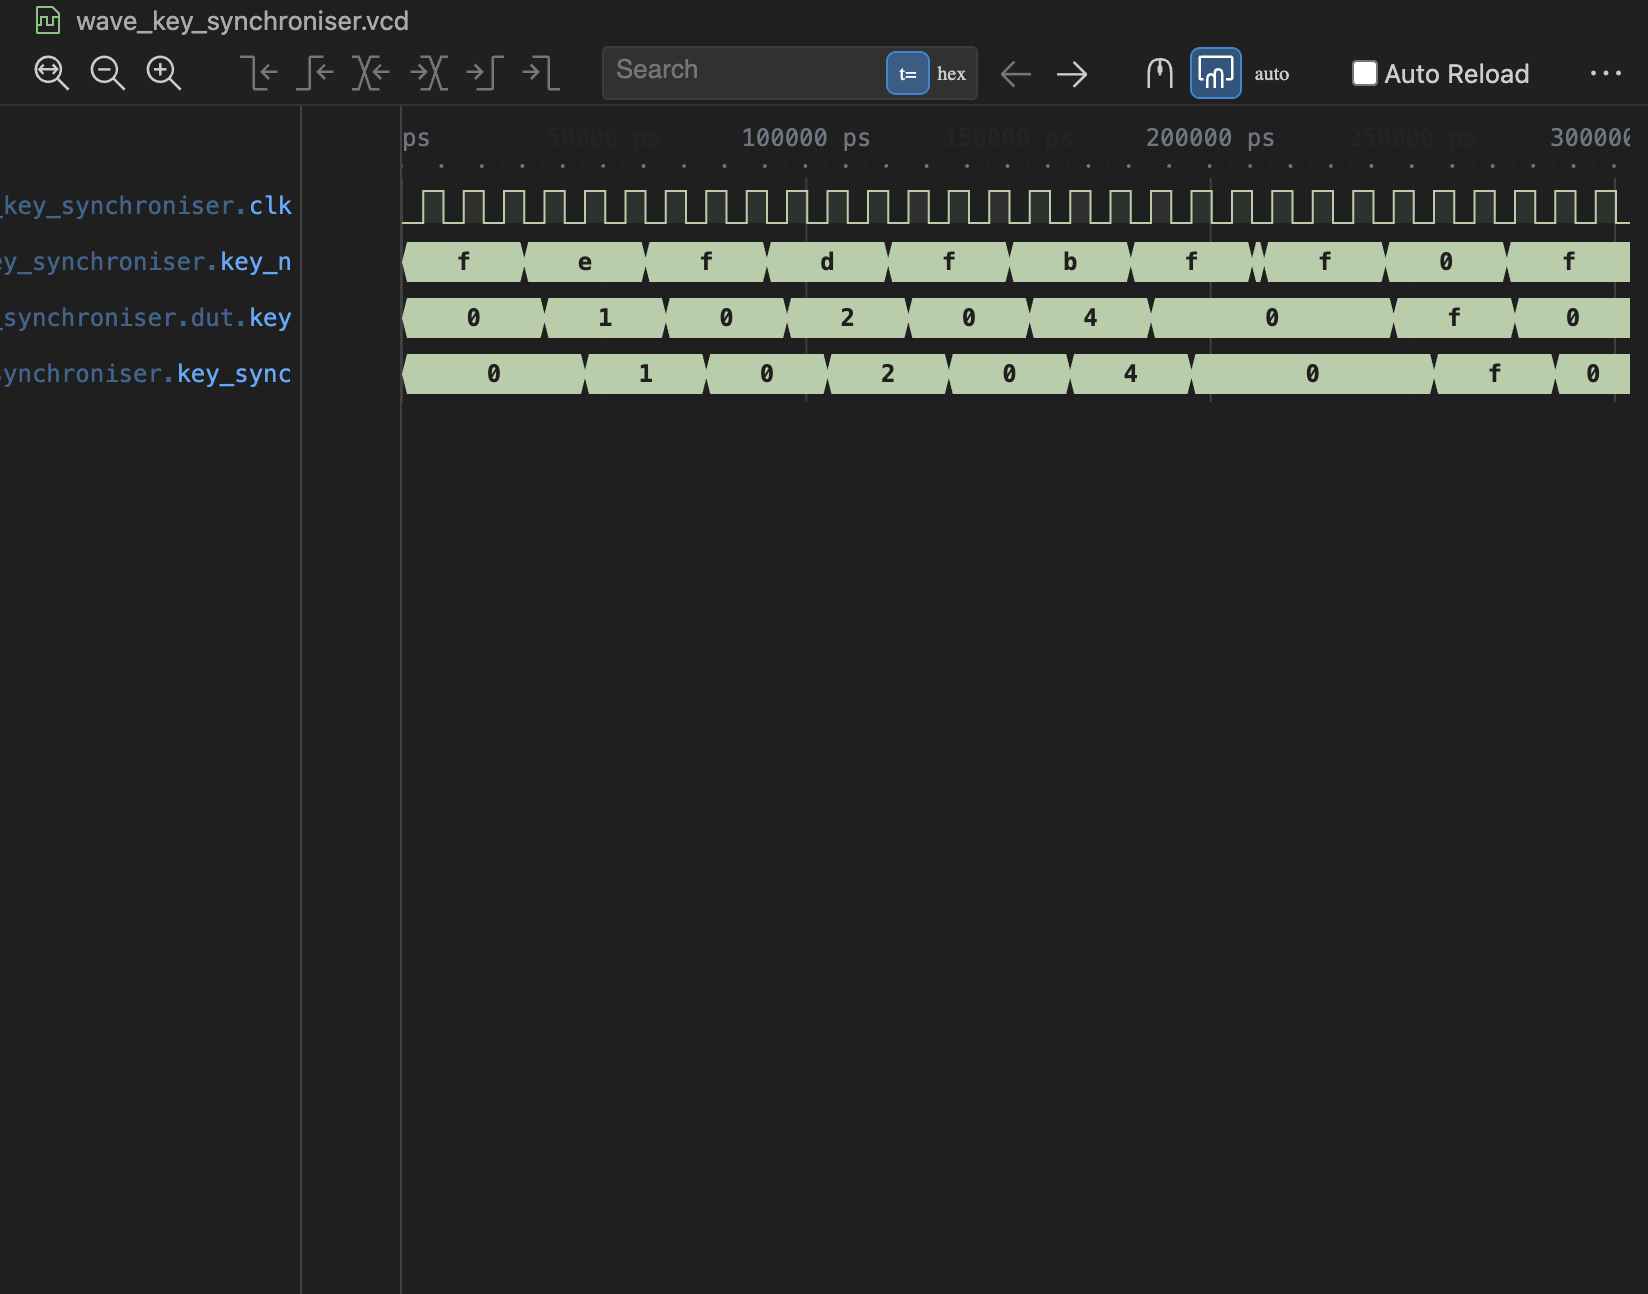
\includegraphics[width=\linewidth]{Images/key_synchroniser.png}
  \caption{Waveform generated for the key synchroniser.}
  \label{fig:ks}
\end{figure}

\subsection{Module 17: Decimal Display Driver}
\subsubsection{Waveform}
The hexadecimal outputs correctly follow the three value variables 
in figure \ref{fig:ddd}. As the blank signals are pulled high the 
hexadecimal digits connected to the blank signal display '7F' which 
is the correct hexadecimal to describe all segments as off for an 
active low hex display. 
\begin{figure}[H]
  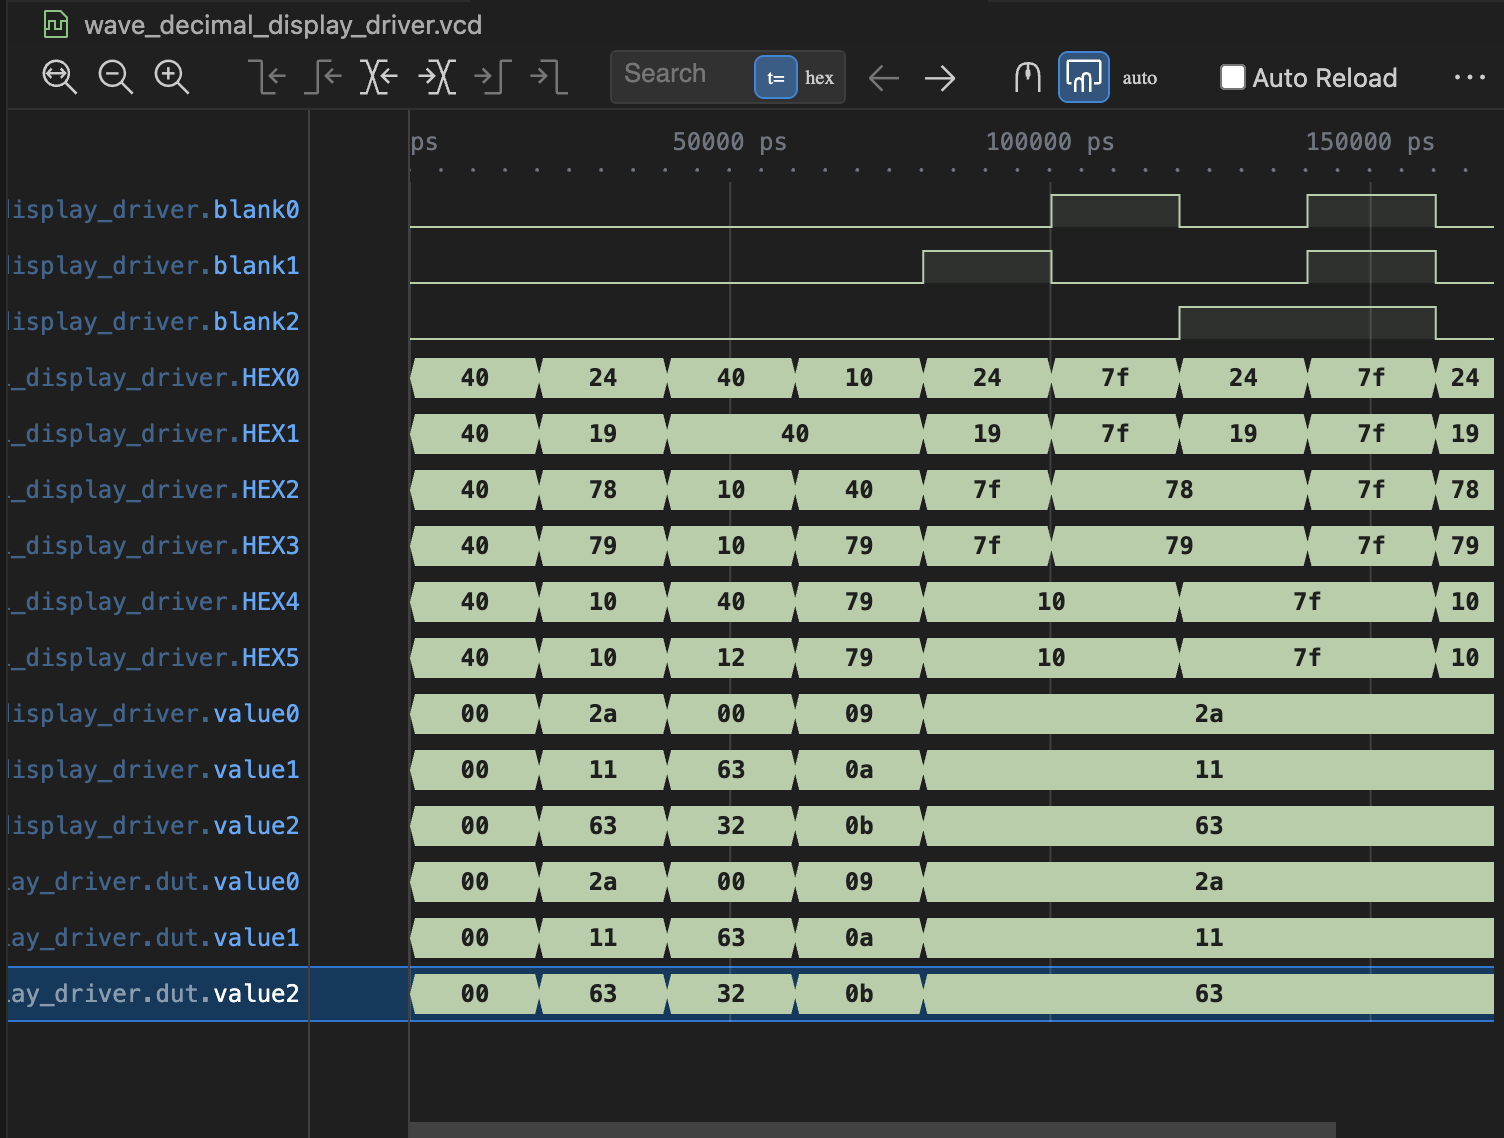
\includegraphics[width=\linewidth]{Images/decimal_display_driver.png}
  \caption{Waveform generated for the decimal display driver.}
  \label{fig:ddd}
\end{figure}

\subsection{Module 18: User Top Watch V1}
\subsubsection{Waveform}
Note that signals temporarily assigned to low for this simpler module 
have been excluded for simplicity.
The 'disp' outputs demonstrate the incrementing behavior of the seconds 
counter which reaches a value of 59 before incrementing the minutes timer 
on the same clock cycle (as seen in \ref{fig:utwo}). This behavior is 
repeated as the minute\_disp signal successfully increments to 2.
\begin{figure}[H]
  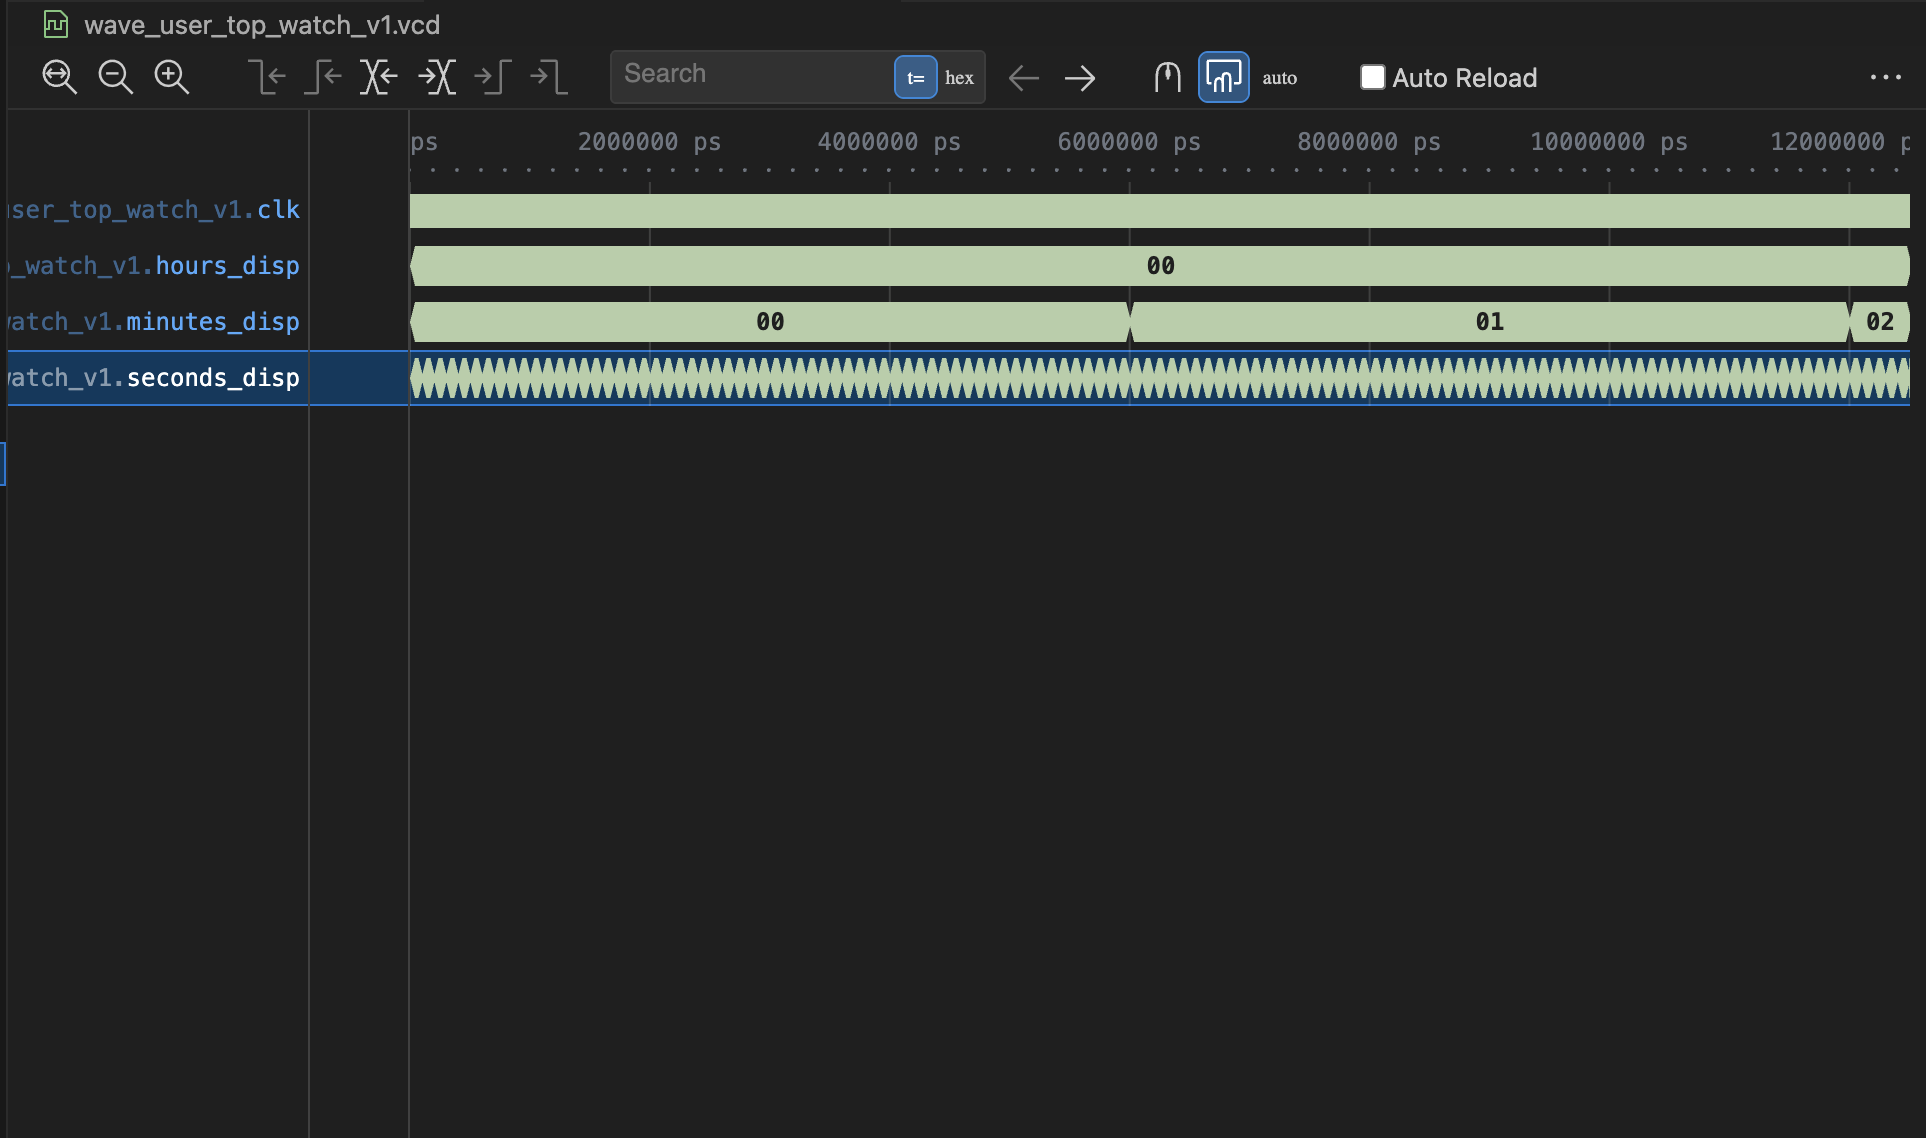
\includegraphics[width=\linewidth]{Images/user_top_watch_v1.png}
  \caption{Waveform generated for the first user top watch module.}
  \label{fig:utwo}
\end{figure}

\subsection{Module 19: User Top Watch V2}
\subsubsection{Waveform}
Note that signals not being tested have been deliberately excluded 
for 
simplicity. The intitial state of figure \ref{fig:utwt} has the blank signals are held low 
and button[3] (8 in decimal) has not been pressed. Button[3] is the 
held for 50 cycles which triggers the edit mode, seen by the switch 
in the mode\_enable signal. This causes the PWM signal to pull the 
seconds\_blank signal low and high accordingly. Two more brief button 
presses switch the mode to minute and hour edit modes, where the minute 
and hour blanking signals follow the PWM signal accordingly.
\begin{figure}[H]
  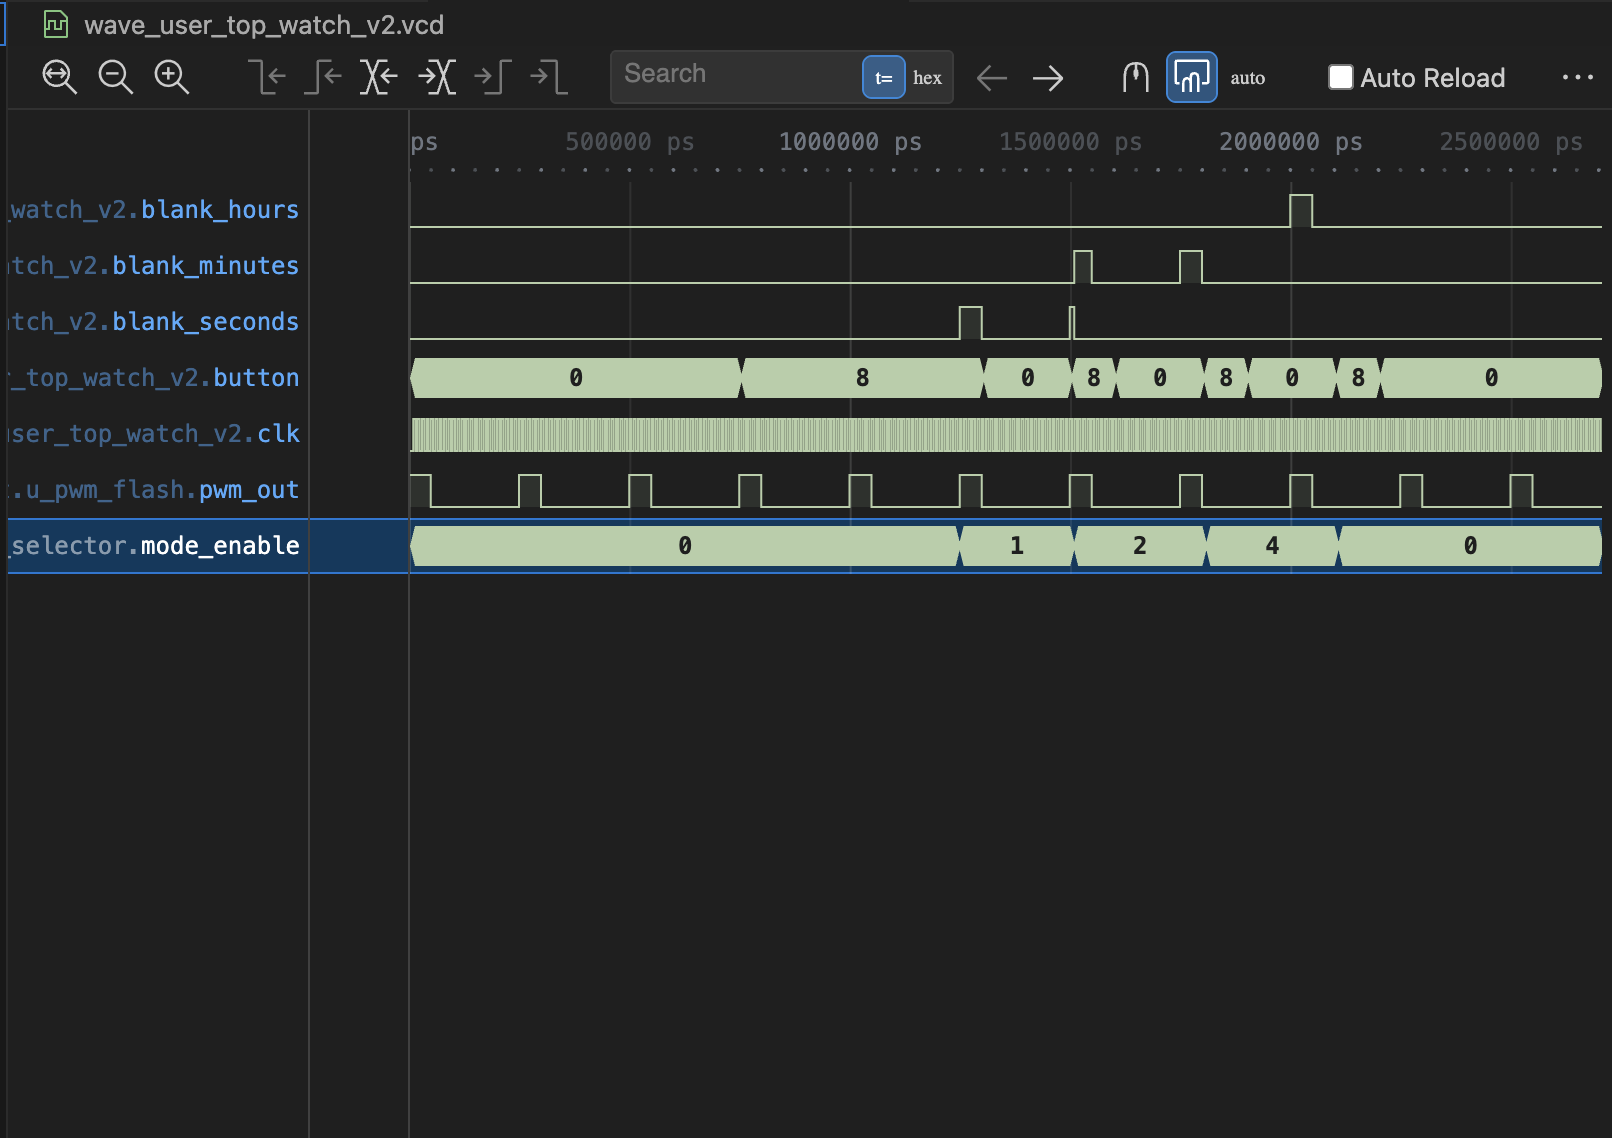
\includegraphics[width=\linewidth]{Images/user_top_watch_v2.png}
  \caption{Waveform generated for the second user top watch module.}
  \label{fig:utwt}
\end{figure}

\subsection{Module 20: User Top Watch V3}
\subsubsection{Waveform}
Note that signals not being tested have been deliberately excluded 
for simplicity. The intitial state of figure \ref{fig:utwth} has the 
seconds counter incrementing by one unit every second (or simulated 
second defined by CYCLES\_PER\_SECOND). This does not change until 
button[3] is held long enough to enter edit mode (decimal 8). As the 
increment button (decimal 2) is pressed, the seconds count increments 
by one unit. If the increment button is held for 0.5s (as defined by the cycles 
per second) the seconds counter begins rapidly increasing. It is further 
demonstrated that a single pulse from the decrement button (decimal 1) 
decreases the second count by one. This behaviour is then tested and 
verified for the minutes and hours counters.
\begin{figure}[H]
  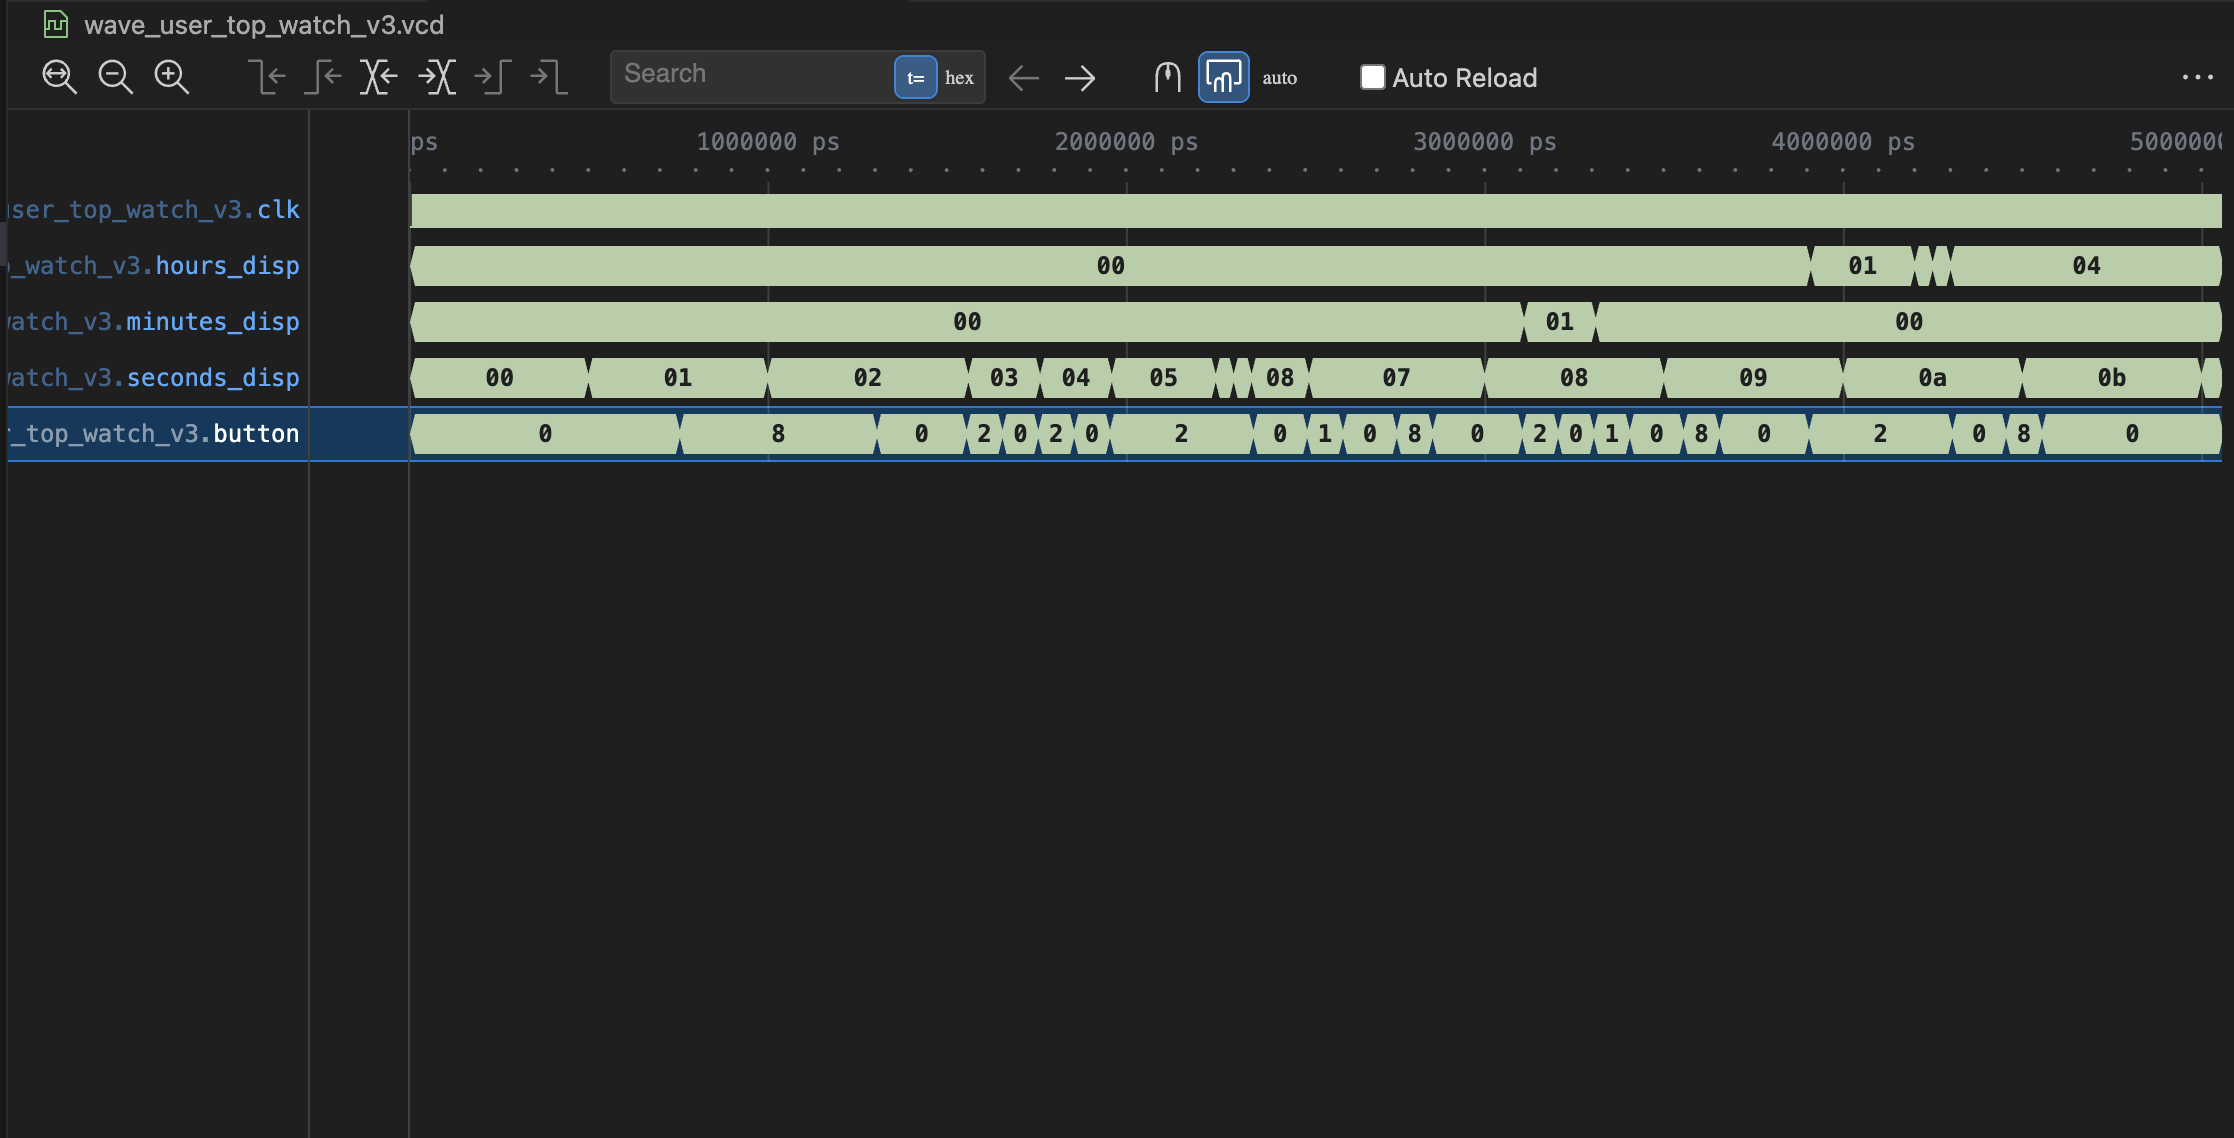
\includegraphics[width=\linewidth]{Images/user_top_watch_v3.png}
  \caption{Waveform generated for the third user top watch module.}
  \label{fig:utwth}
\end{figure}

\subsection{Module 21: User Top Watch V4}
\subsubsection{Waveform}
Note that signals not being tested have been deliberately excluded 
for simplicity. The intitial state of figure \ref{fig:utwf} has no 
input, which results in the seconds counter incrementing normally. 
Button[3] (decimal 8 on the button signal) is held down to bring the 
mode\_enable signal to 1 (seconds edit mode). In this state, the seconds 
counter no longer increments, which is the expected behavior for the 
v4 additions. Once button[3] has been pressed again, the mode\_enable signal 
is set to 2 bringing the system out of seconds edit mode. At the next 
seconds clock pulse, the seconds counter increments again demonstrating 
that the defined behavior from the v1 to v3 has not been altered.
\begin{figure}[H]
  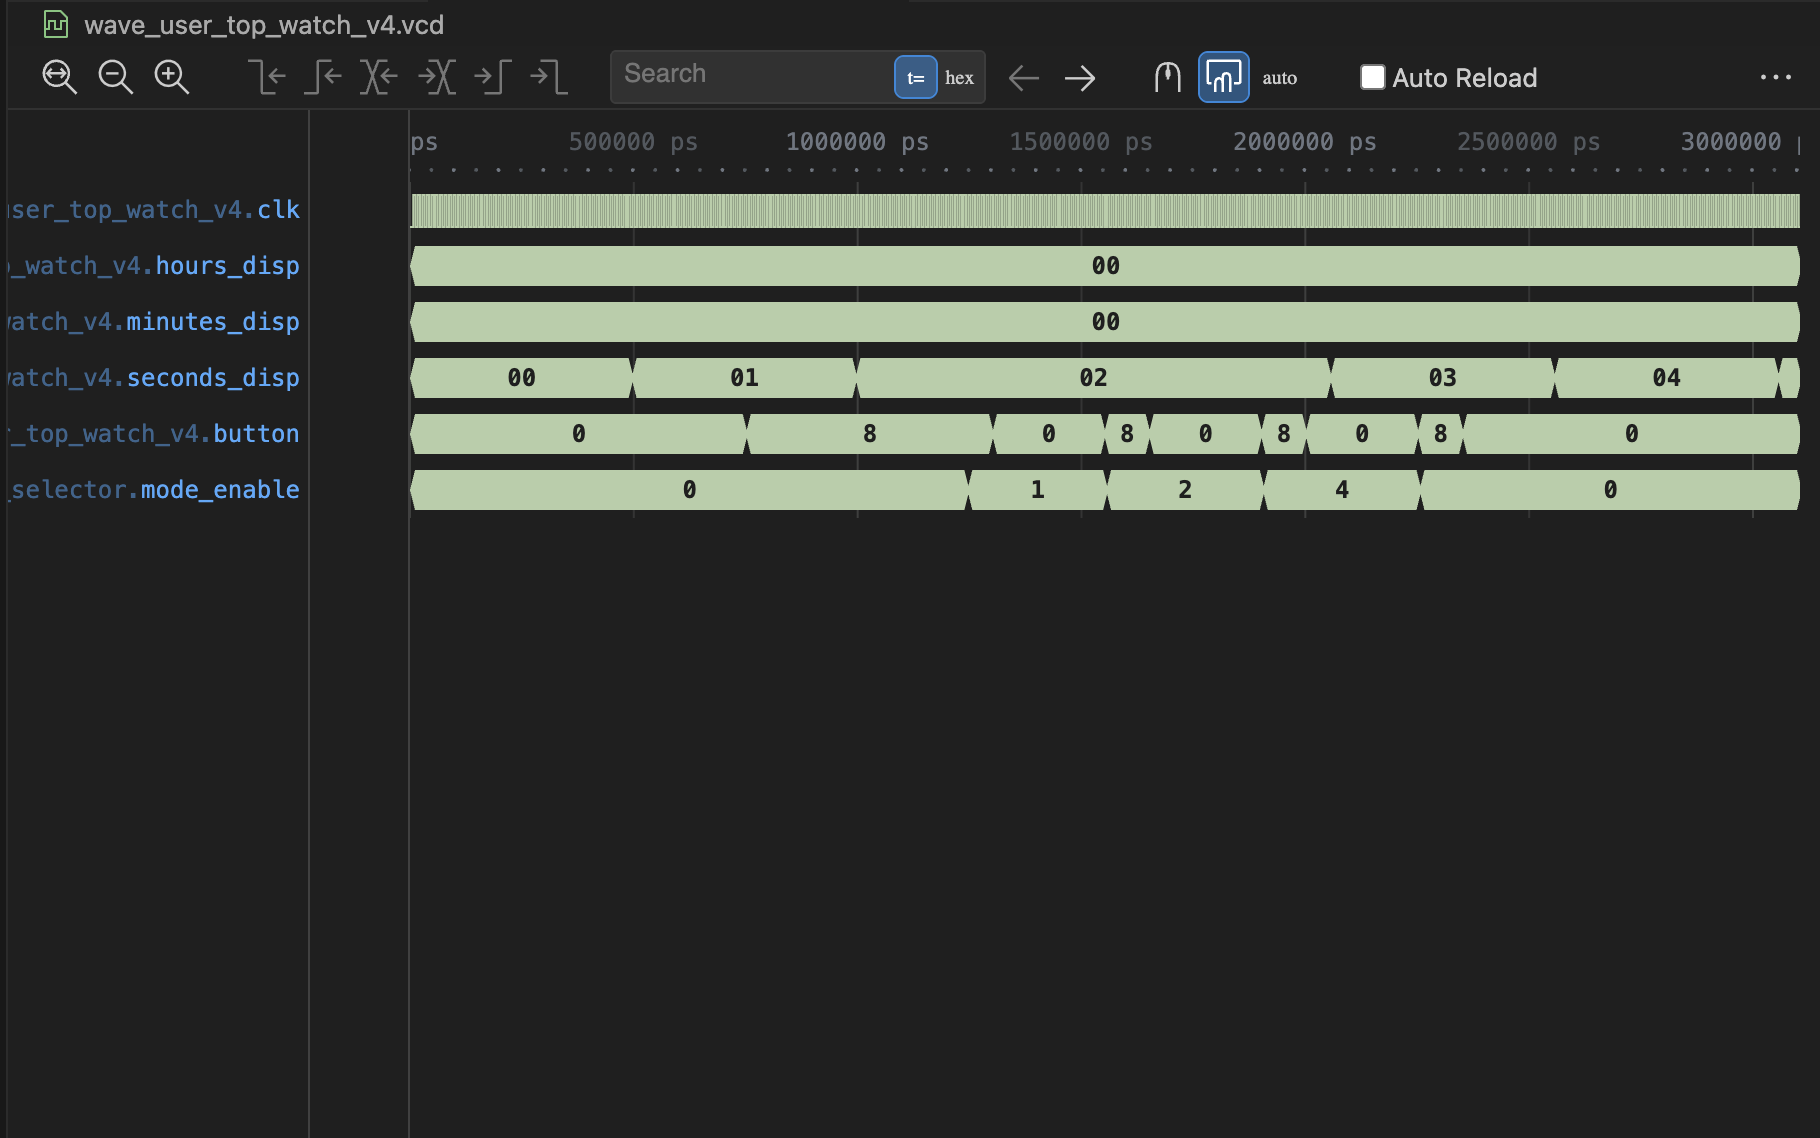
\includegraphics[width=\linewidth]{Images/user_top_watch_v4.png}
  \caption{Waveform generated for the fourth user top watch module.}
  \label{fig:utwf}
\end{figure}

\section{Assignment 2 Modules}
This section covers the function and testing of each module in 
the assignment 2 portion of the project (The rest of the project).
\pagebreak

\subsection{Module 22: Cascade Counter}
\subsubsection{Description}
The cascade counter module is a generalised HMS counter with no edit function. 
As it is only required for the stopwatch, it must only count up. Editing the 
time would beat the point of the stopwatch (ex. 3s 100m sprint times).

\subsection{Module 23: Stopwatch Counter}
\subsubsection{Description}
The stopwatch counter is a specialised implementation of the cascade counter 
that counts in minutes, seconds and centiseconds and is driven by a 
centisecond restartable rate generator.

\subsection{Module 24: Snapshot Multiplexer}
\subsubsection{Description}
The multiplexer takes in a register of signals, and stores the current input 
signal in an internal register. Under normal operation the input is linked
combinationally with the output. When the hold signal is pulled high the 
module stops updating the internal register and the output reflects the internal
register.

\subsection{Module 25: Stopwatch Control}
\subsubsection{Description}
This module defines a moore FSM for the different stopwatch functions to fit the 
given specification (listed below).
\begin{verbatim}
  // Pressing start stop toggles stopwatch b/t running and stopped
  // If running with live display, lap freezes the display
  // If running with a frozen display, lap unfreezes the display
  // If stopped with a frozen display, lap unfreezes the display (no rst)
  // While stopped with a live display, lap resets time to 0
  // If both buttons are pressed, then both are ignored
\end{verbatim}

\subsection{Module 26: User Top Stopwatch Version 1}
This module is prototype. The test cases were successful. Further documentation 
will be saved for the final module. 

\subsection{Module 27: User Brightness Wrapper}
Module sucsesfully modulates blank signals according to PWM specifications. 
All test cases in both SBY and Pytest have been passed.

\subsection{Module 28: User Top Timepiece V1}
Module succesfully insantiates and operates modules. Module passed required 
testing.

\subsection{Module 29: User Top Brightness Timepiece}
Module succesfully insantiates and operates modules. Module passed required 
testing.

\section{Assignment 1 Questions}

\subsection{Report 1}
Blank is a 1 bit wide logic signal, while ACTIVE LOW is defined as 
an integer, which is a multi-bit data type (32 by default) which will 
throw a warning if truncated.

\subsection{Report 4}
BCD is a method of encoding decimal bits in binary that reserves a 
number of bits (usually 4 for 0-9) for each decimal digit, before 
concatenating all of the digits into a single register. Storing the 
digits individually provides greater accuracy at high counts, and helps 
to avoid rounding errors making it a common tool in precision counters.

\subsection{Report 5}
The code uses the clog2 function, which takes the ceiling of the log2
operation on the number of cycles. This ansers the question of " how
many powers of 2 ($2^n$) do I need to have a number greater than the cycle
count?". As the maximum number stored in a set of bits also expands
such that the maximum storeable number is $2^n$ where n is the result
of clog2, this statement produces the minimum number of bits required 
to store the cycle count in a register.

\subsection{Report 6}
The code used for the testbench was stored in 
waverestartable\_rate\_generator\_one.v and produced the output in
wave\_restartable\_rate\_generator\_one.vcd. The code is a direct
modification of wave\_restartable\_rate\_generator\_one.v, using
a CYCLE\_COUNT of 1.

\begin{verbatim}
// Wave restartable rate generator testbench for max cycle of 1 case
// Based of wave_restartable_rate_generator.v written by Jonathan Manton
//
`timescale 1ns / 1ps

module wave_restartable_rate_generator_one;
  reg  clk = 0;
  reg  run = 0;
  wire tick;

  restartable_rate_generator #(
      .CYCLE_COUNT(1)
  ) dut (
      .clk (clk),
      .run (run),
      .tick(tick)
  );

  always #5 clk = ~clk;

  initial begin
    $dumpfile("wave_restartable_rate_generator_one.vcd");
    $dumpvars(0, wave_restartable_rate_generator_one);

    // Run: tick fires every CYCLE_COUNT clocks
    #30;
    run = 1;
    #130;

    // Disable mid-cycle: counter resets, no stray tick on re-enable
    run = 0;
    #30;
    run = 1;
    #90;

    run = 0;
    #20 $finish;
  end
endmodule
\end{verbatim}

The code produced the wave table in figure \ref{fig:rrgo}.
\begin{figure}[H]
  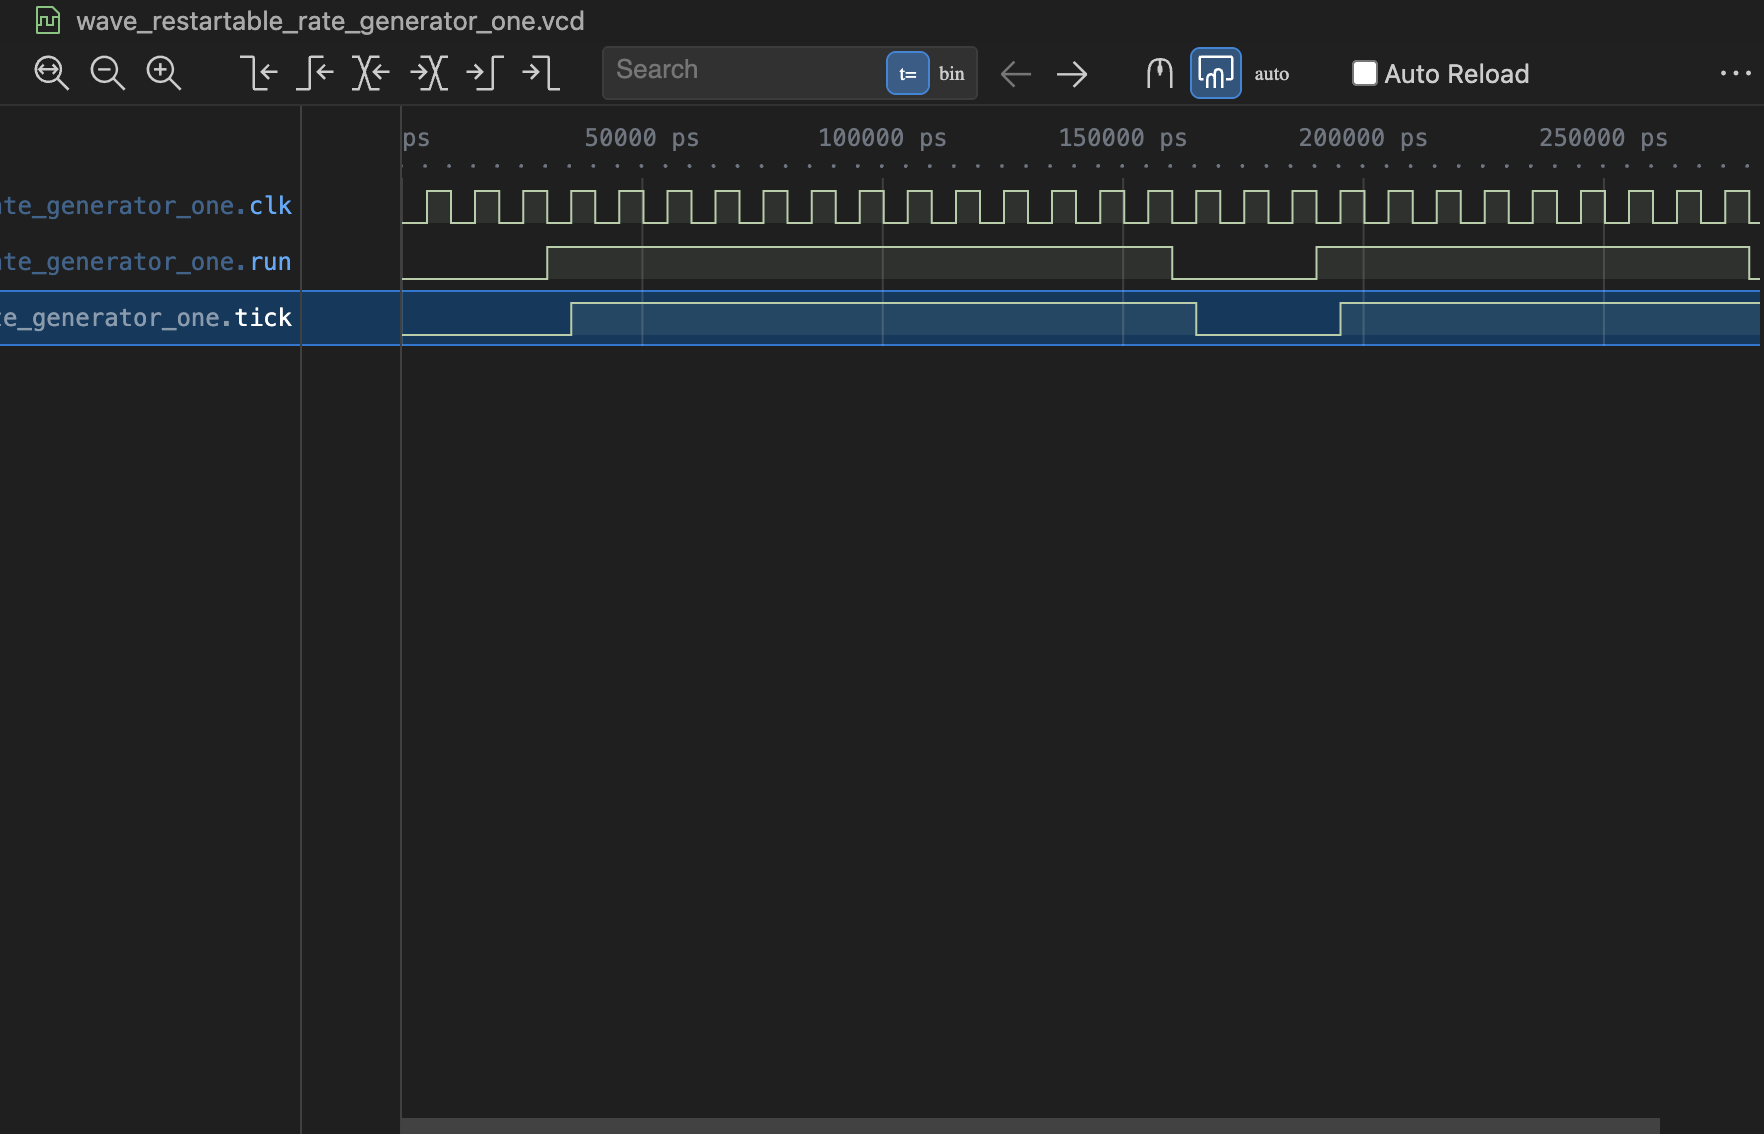
\includegraphics[width=\linewidth]{Images/restartable_rate_generator_one.png}
  \caption{Waveform generated for the mod n counter.}
  \label{fig:rrgo}
\end{figure}

The tick signal remains high while after the run variable is high 
(and has settled), which is the correct special specified behaviour 
for the case where CYCLE\_COUNT = 1.

\subsection{Report 7}
The module name can be lengthened to pulse width modulation 
generator, which describes the modules real purpose. The module 
produces a signal with a specified on and off time over a period, 
usually to controll the amplitude of a connected device (as the 
average signal can be raised or lowered depending on how long the 
signal is on or off, otherwise known as the duty cycle). This allows 
for specific voltage control without using a digital to analog 
converter.

\subsection{Report 8}
It allows for the rst signal to be used as a form of enable function,
keeping the counter at 0 while it is high. In the PWM generator module
this provides an easy way to pause the counter and reset the PWM cycle 
at the same time.

\subsection{Report 9}
As the output is a function of the current state, feeding the next 
state logic with the output logic is still equivelant to just processing 
the current state using more complex next state logic, therfore the system
is still a Moore FSM.

\subsection{Report 10}
Figure \ref{fig:bhp} contains the waveform produced by the module. The 
module utilises the button\_hold\_detect module which pulls the output high 
once the input button has been pressed for a specified number of clock cycles. 
The continuous high output of the detect module is wired to the rising 
edge detector module, which converts a rising edge into a once cycle wide 
pulse signal, which is the desired output for this module.

\subsection{Report 11}
While the rising\_edge\_detector module is a mealy FSM (as the high / 
pulse output is dependant on a rising edge input), it is implemented as 
part of the next state logic in this module. When looking at the inputs and 
outputs of the button\_hold\_pulse module, the button and clk signals 
only drive the two sub-modules, and are not used to assign an output directly, 
which makes this module a Moore FSM rather than a Mealy.

\subsection{Report 12}
STILL NEED TO COMPLETE

\subsection{Report 13}
The two types are handled differently at a compiler level (logic 
being considered a variable along with int, bit etc. while wire is a net 
data type). In this case, the wire net type specifies that a signal can 
be driven by multiple sources, therefore the wire net type (that automatically 
implies a logic type) allows the logic signals to be driven by multiple 
sources in this code. 

\subsection{Report 14}
Proper testing of the system on the board would take at least 48 hours 
to confirm two correct cycles of the board. This is assuming that there 
was no debugging required when compiling the code in Quartus. In reality 
each iteration could take 3 days to properly test along with lab equipment 
to capture the behavior of the board on camera for the complete test 
time. This would be completely impractical to complete for every version 
of the software.
\break
\break
The automated test suite allows the programer to fail early and 
inexpensively as the test suite can catch bugs even at the basic 
testing phase of the project (as long as the behavior has been 
defined prior to testing). By catching errors at the first stage of the 
project, the programer can be confident that any errors encountered in 
the next stage are a result of the changes, and not the original code. 
This reduces the volume of code a programer has to search through for a 
bug making big fixes in subsequent versions much quicker.
\break
\break
The test would take significantly longer to run for the same time 
period as there are more clock cycles to consider, and therefore more 
calculations that need to be completed to test the modules ( note that 
this does not apply for step based testing, which will simply complete 
faster). With this in mind, it is important to write testable code with 
opportunities to redefine clock cycles in order to quickly simulate the 
modules.

\subsection{Report 15}
Relevant waveforms have been chosen for the top timer report sections. 
to verify this, see sections 0.2.18 to 0.2.21. Relevant waveforms 
include only waveforms of direct effect or of direct consequence of the 
elements being tested. 

\subsection{Report 16}
Assuming reset refers to the run function of the restartable rate 
generator, the design produces on one continuous reset for each time 
that the system is brought into the seconds editing state. This is 
not a problem as the run port is defined to hold the rate generator 
at it's current state if pulled low, therefore there is no need for 
multiple resets and adjustments of the rate generator keep the 
value correct without incrementing.

\subsection{Report 17}
It was very rare in the labs to achieve the correct function on the 
first test of module. Often details like next state logic or even 
variable names were mixed up which forced another 5 minute recompile 
cycle. The Visual Studio Code environment combined with pytest is a much 
more efficient method to program the modules as the compiler is quick, 
and the quality of life features such as real time linting make the 
development process significantly quicker. Not to mention the improved 
module accuracy when using automated test suites that catch small 
details such as clock cycle misalignment. For these reasons, I much prefer 
working in the Visual Studio Code environment.

\subsection{Report 18}
A deviation value of 50PPM means that at it's absolute maximum, the 
clock can deviate by 50 clock cycles for every 1 million clock cycles.
Equation (1) is a calculation displaying the absolute maximum number 
of clock cycles out the De1-soc can become over a 24 hour period.
\begin{equation}
  (50PPM) \times 50 (MHz) \times (24 \times 60^2) = 216000000(cycles)
\end{equation}
Equation (2) converts the clock cycles into seconds.
\begin{equation}
  \frac{216000000(cycles)}{50,000,000(MHz)} = 4.32(S)
\end{equation}
Therefore the maximum drift is 4.32 seconds. Note that this maximum 
drift is an absolute worse case scenario. In most cases, the clock 
will drift both forward and backward, resulting in a fraction of the 
drift per day.

\section{Assignment 2 Questions}

\subsection{Report 1}
It would also be possible to possible to alter every instance of the 
counter by surrounding by adding a new reset function, or branching 
the project off completely to create a new version. Both of these options 
are far more impractical than the ones mentioned by the question. As the module 
is already referenced many times in code, altering the original file would require 
re-writing many other modules, which would all have to be retested and verified. 
The thin wrapper approach may work, but would be unessacary given that all of the 
previously written code will refer to the original module while all the new 
code will refer to the new module. There is no time or resources saved when compared 
to copying the file and renaming it. Therefore it would be best to copy the 
module and rename it, altering only the new file.

\subsection{Report 2}
The assertions cover all reasonable behavior whether explicitly such as the 
parameter checks or implicitly, such as the maximum value being 
verified as part of the wrapping checks. With this in mind 
the verification must be run long enough (multiple full count 
cycles for both the count up and count down functions ) in order 
to check that all conditions are met (eg. wrapping conditions don't 
happen every clock cycle).

\subsection{Report 3}
To verify the module for all values of MAX, the module must be checked 
with formal mathematical verification. Mathematical proof is the 
only method that can prove a process true for all input values rather than 
for specific test runs.

\subsection{Report 4}
Figure \ref{fig:udcr} demonstrates that an invalid value of 62 was used as 
an initial state for the test. This prevented the counter from incrementing 
once it was enabled therefore failing the count increment assertion on line 63 
of the assertion file. By restoring the count <= MAX assertion, 62 
would be considered an invalid starting case therefore would not 
constitute a valid base case for a formal proof, invalidating the failure. 
\begin{figure}[H]
  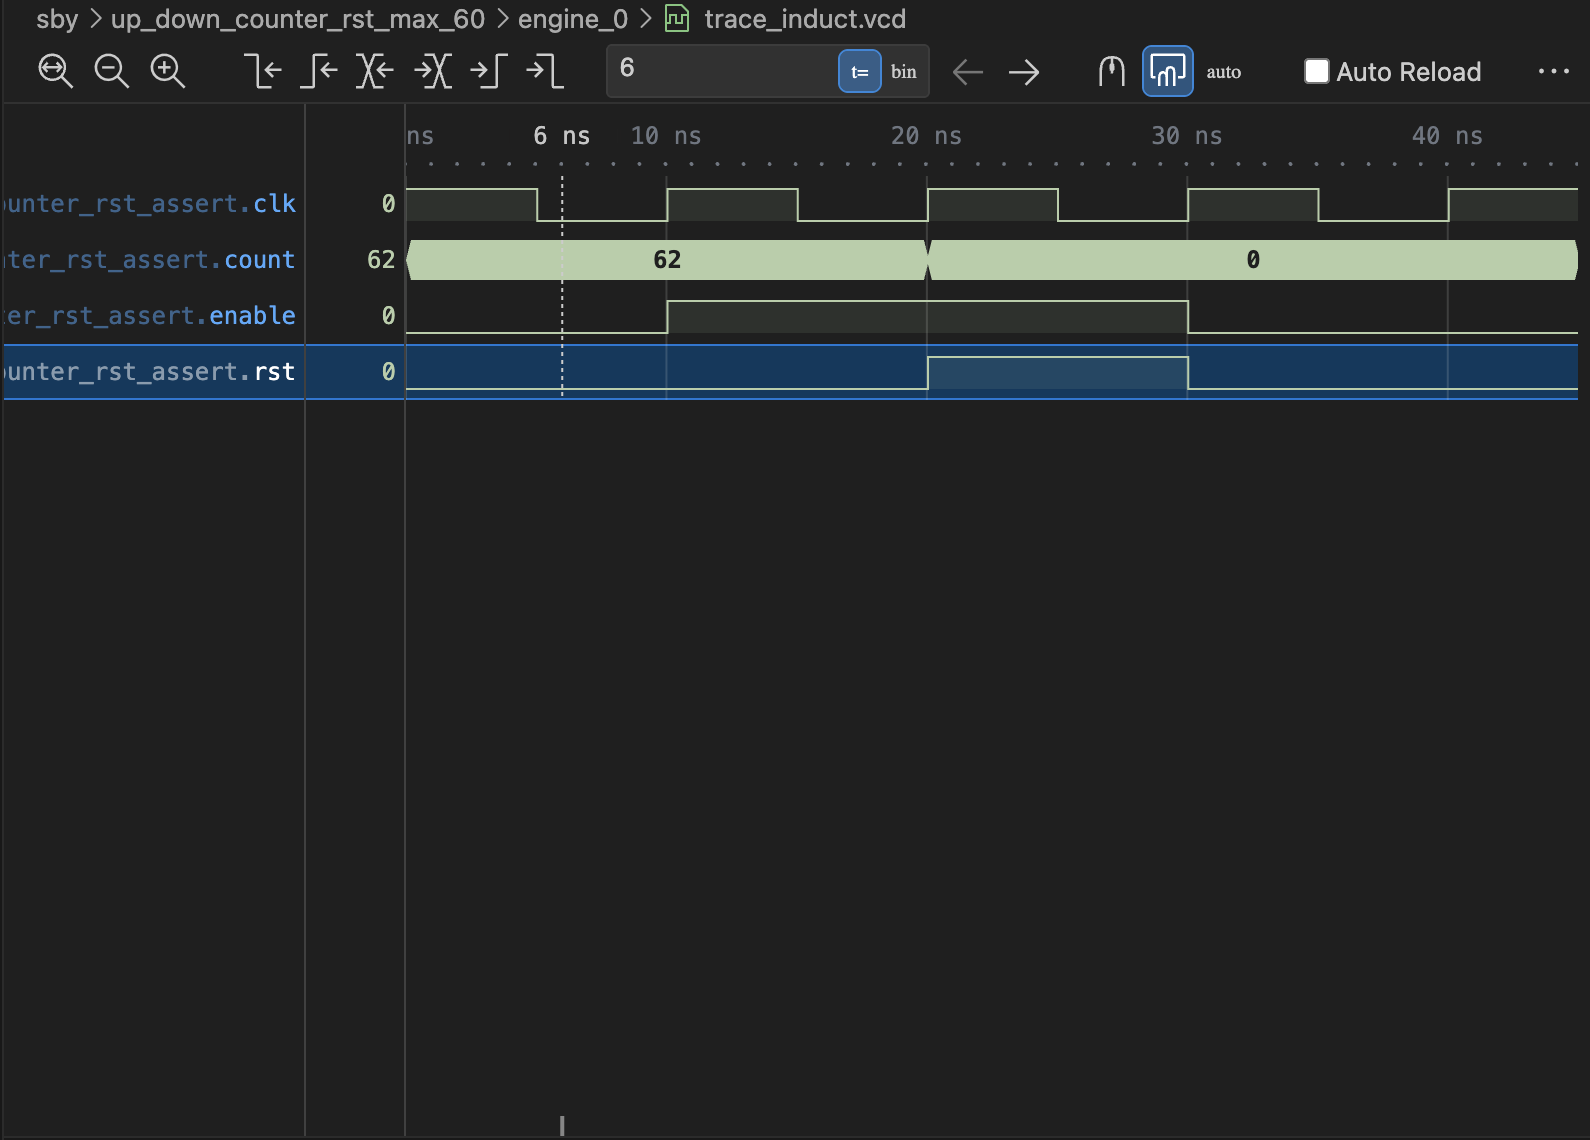
\includegraphics[width=\linewidth]{Images/up_down_counter_reset.png}
  \caption{Waveform generated as a counterexample to formal verification.}
  \label{fig:udcr}
\end{figure}

\subsection{Report 5}
YET TO BE COMPLETED. WILL DO ONCE I'VE FINALISED THE DESIGN.

\subsection{Report 6}
At its most basic function, the stopwatch is a series of cascading counters for the seconds, 
minutes and hours with a secondary counter to track the laps. This base layer 
is responsible for basic counting functions and registers. 
\break
The next layer connects the seconds, minutes and hours timers together with a 
rate generator set to time seconds. This is supplemented with the correct rollover logic.
 This layer is responsible for correct timekeeping.
\break
The next layer handles the lap function, taking snapshots of the time and storing them in 
the correct register. This layer is responsible for the lap logic.
\break
The next layer handles the stop, start and lap logic and connects these button inputs 
to ports such as reset and enable. This layer is responsible for the correct 
input logic and timer function. 
\break
The top layer handles decimal to display conversions and display features. This 
layer is responsible for displaying information in a readable and useful way.

\subsection{Report 7}
YET TO BE COMPLETED. REQUIRES DRAWING.

\subsection{Report 8}
The enable signal of the counter is decided using the combinational logic 
\verb|tick && enable|. STILL NEEDS TO BE FILLED OUT, QUESTION NEEDS 
CLARIFICATION.

\subsection{Report 9}
YET TO BE COMPLETED. REQUIRES DRAWING.

\subsection{Report 10}
YET TO BE COMPLETED. REQUIRES DRAWING.

\subsection{Report 11}
The borrow complement signal is generated with a NAND gate, of which the inputs are: NOT down, 
NOT output A, NOT output B, NOT output c and NOT output D. The BO signal will only
turn off when the down function is off, and the counter is at 0. As the borrow complement signal 
represents a counter underflow (to trigger another chained counter IC to increase the 
number of counter registers), the schematic is saying that the BO (borrow) complement signal should 
only go low when the down signal is not high, and the counter is at 0. As we are interested 
in the borrow signal not the borrow complement signal, then we are looking for the inverse of 
this behavior. 

\subsection{Report 12}
The first section implemented was the basic countdown and cascade counting 
feature set. This involved instantiating a restartable rate generator and 
three editable countdown modules where the borrow signal was used to tick the 
subsequent counter module. Next, the states were defined as local parameters and 
the next state logic was implemented. This also includes instantiating an edit 
mode selector, as the output was required in the next state logic.
\break
\break
The next step involved instantiating a rising edge detector for the state change 
button (button[0]) and two button auto repeats for the incrementing and 
decrementing buttons. These were linked to the counter modules.
\break
\break
Finally, with a range of modules instantiated, the assignmnets were described at 
the bottom of the module, most of which were copy pasted from the user\_top\_watch\_v4. 

\subsection{Report 13}
The states were chosen to be Stopped, Running and Set, with minute set, hour set 
and second set being sub-states of the Set state. As the states were decided early 
in the design of the module, a simple binary state encoding was chosen to mirror 
forms seen earlier in the course. This has the added advantage of minimising flip 
flops.
\break
\break
From the stopped state (default), the increment of the edit substate pushes the 
state into set. However if the start button is pressed then the state will change 
to running. From the running state, pressing the start button will push the state 
into stopped. From the set state, the edit substate returning to 000 will push the 
system back to the stopped state.

\subsection{Report 14}
The exact specification for each model and exact testing for each model meant I 
had certainty that my previous work would hold up to future scrutiny in more 
complex modules. It also meant that my code itself was documentation and 
required only a small portion of written documentation. This made it easy to 
debug and test modules later down the line as I found issues in parent modules. 
However, the test were often overly specific, and assumed a very specific 
architecture which was not necassarily the only way to complete a task. This 
caused much frustration and time loss. In future, I would take on the task 
of writing tests to fit a simpler solution, or a solution that is more obvious 
to myself. 

\subsection{Report 15}
Given this project took me ~30 hours to complete, I would say VS code and modern 
tools saved me 10 hours. The linting features were a life saver and likely 
saved me 4 hours, as it would take me 3 or 4 lints to remove all errors and 
warnings from each module. Automated tests saved me anywhere from 10 to 20 hours 
as I could have certainty that the code I had written was mostly correct, 
and would not cause an error during the testing of later modules. The same can 
be said for formal verification. Without these tools, the problems I encountered 
would have remained hidden until the top modules of each section, where they 
would have been impossible to debug within the time constraints. 

\subsection{Report 16}
The \$lt cell corresponds to a less than operator, used in the comparison if 
statement that determines whether to reset or continue counting up. The \$add 
cell corresponds to the addition statement in the count case of the if 
statement (next\_count = count + 1). Finally, the \$mux represents a multiplexer 
that switches between A and B (reset and counting modes) using the result of 
the comparison. 
\begin{figure}[H]
  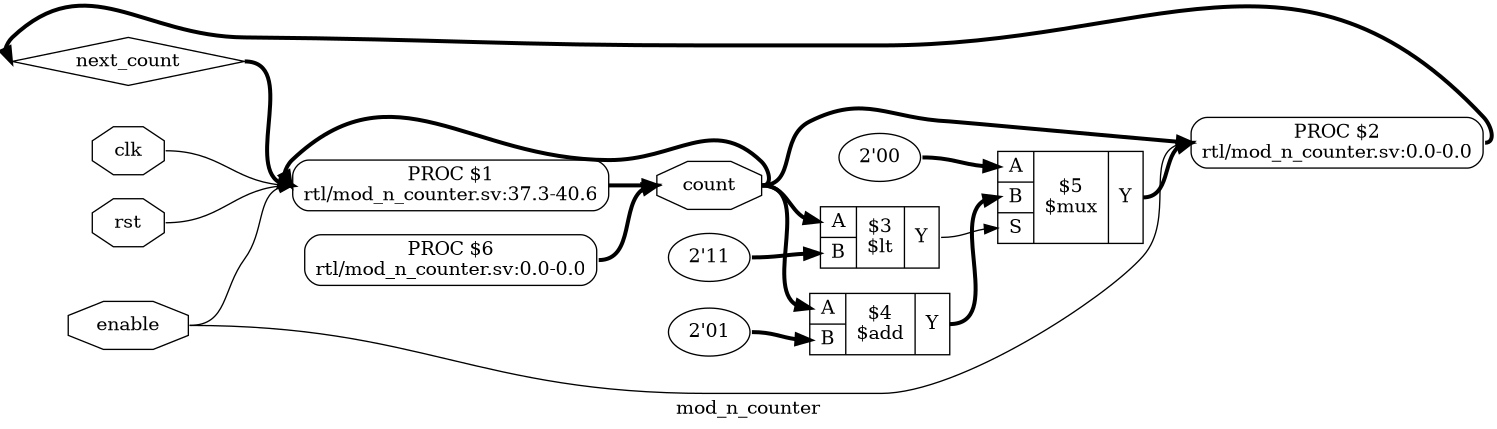
\includegraphics[width=\linewidth]{Images/elaborated.png}
  \caption{Elaborated diagram produced by yosys.}
  \label{fig:eyosys}
\end{figure}

\subsection{Report 17}
\$sdffe is the yosys block for a flip flop with synchronous reset and an enable 
pin. The CLK pin is the system clock input, the D pin is the input, which is 
driven by the next state logic (as seen with the arrow), the EN input is the 
enable signal and SRST is the synchronous reset. The proc command appears to 
have kept combinational logic untouched, but has combined PROC cells into 
appropriate flip flops. 
\begin{figure}[H]
  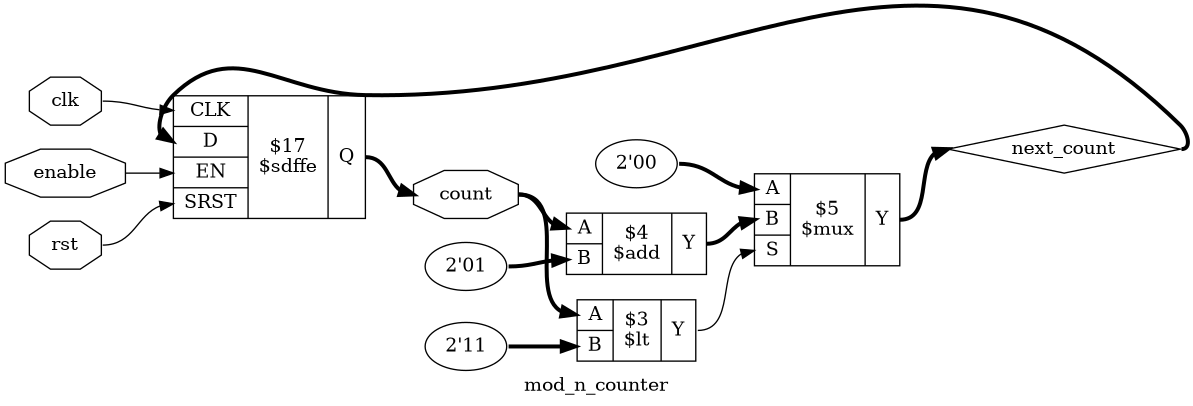
\includegraphics[width=\linewidth]{Images/proc.png}
  \caption{Proc diagram produced by yosys.}
  \label{fig:procyosys}
\end{figure}

\subsection{Report 18}
It is possible that the doubling of flip flips  is a result of the 
initialisation of the count variable. Yosys requires this logic split to 
move the correct logic signals to the correct logic gates. Unlike the cells, 
it is normal for signals from a register to enter a set of logic gates in a non 
seuential order. The PPOP configures four polarity values, the clock trigger 
(P:positive), reset (P:positive), reset value (O:resets to 0) and the enable 
(P:active high).
\begin{figure}[H]
  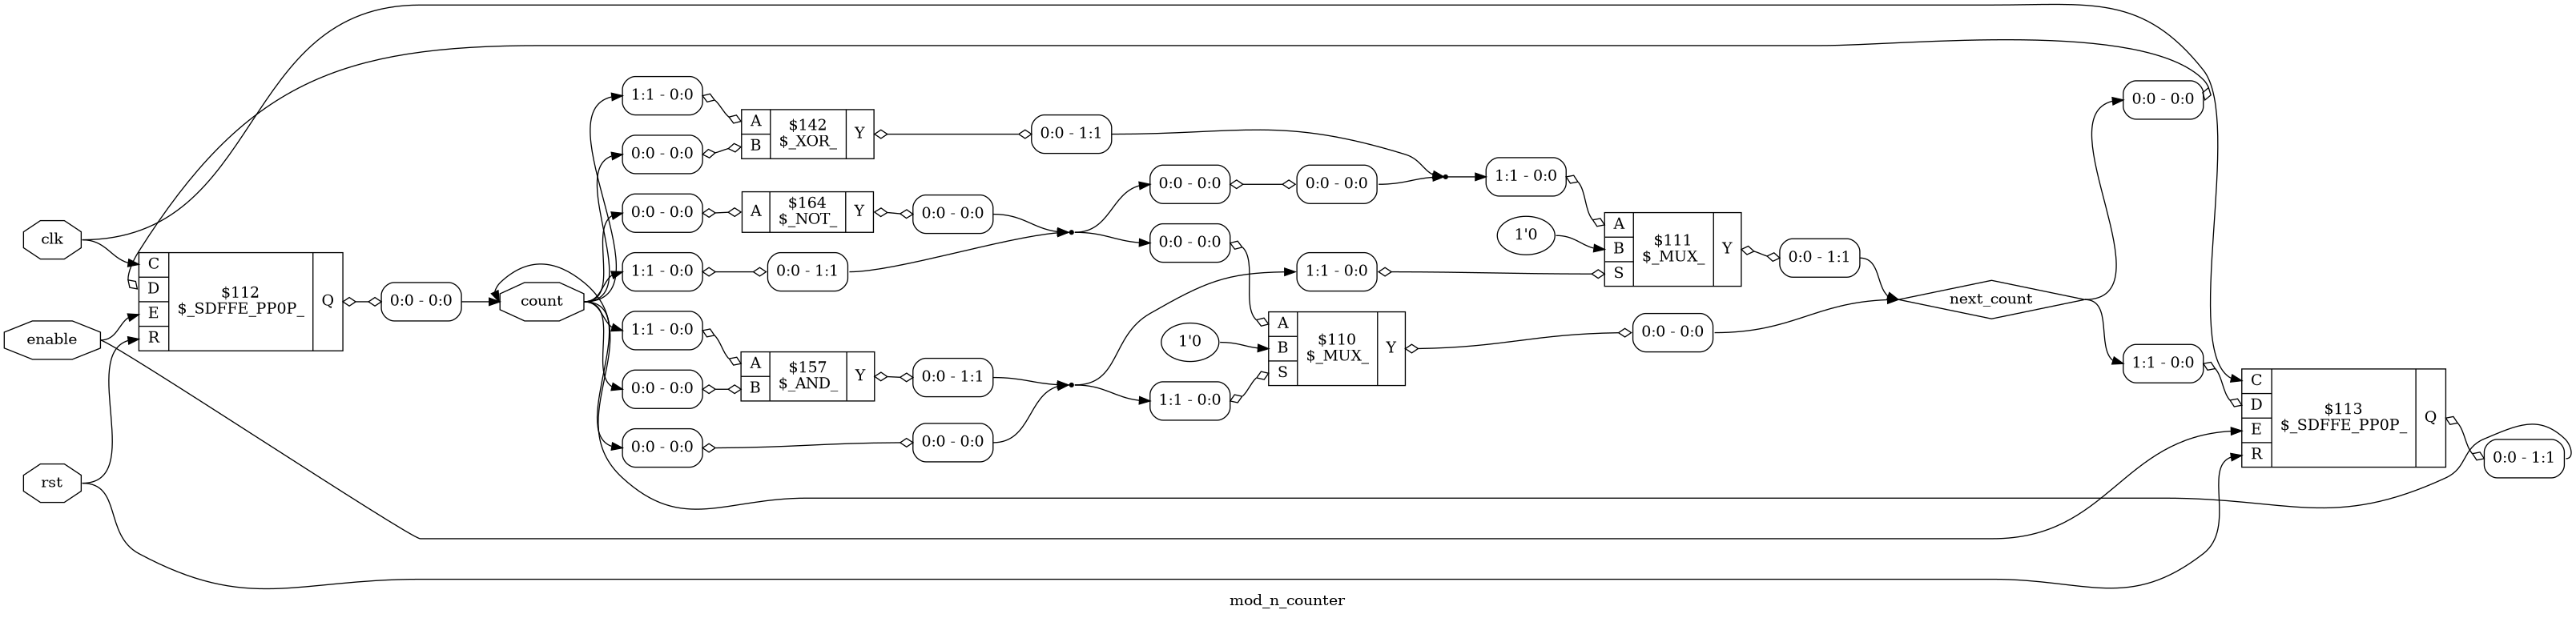
\includegraphics[width=\linewidth]{Images/techmap.png}
  \caption{Techmap diagram produced by yosys.}
  \label{fig:procyosys}
\end{figure}

\subsection{Report 19}
REQUIRES DIAGRAM, LEFT FOR FINAL RUN OVER
\begin{figure}[H]
  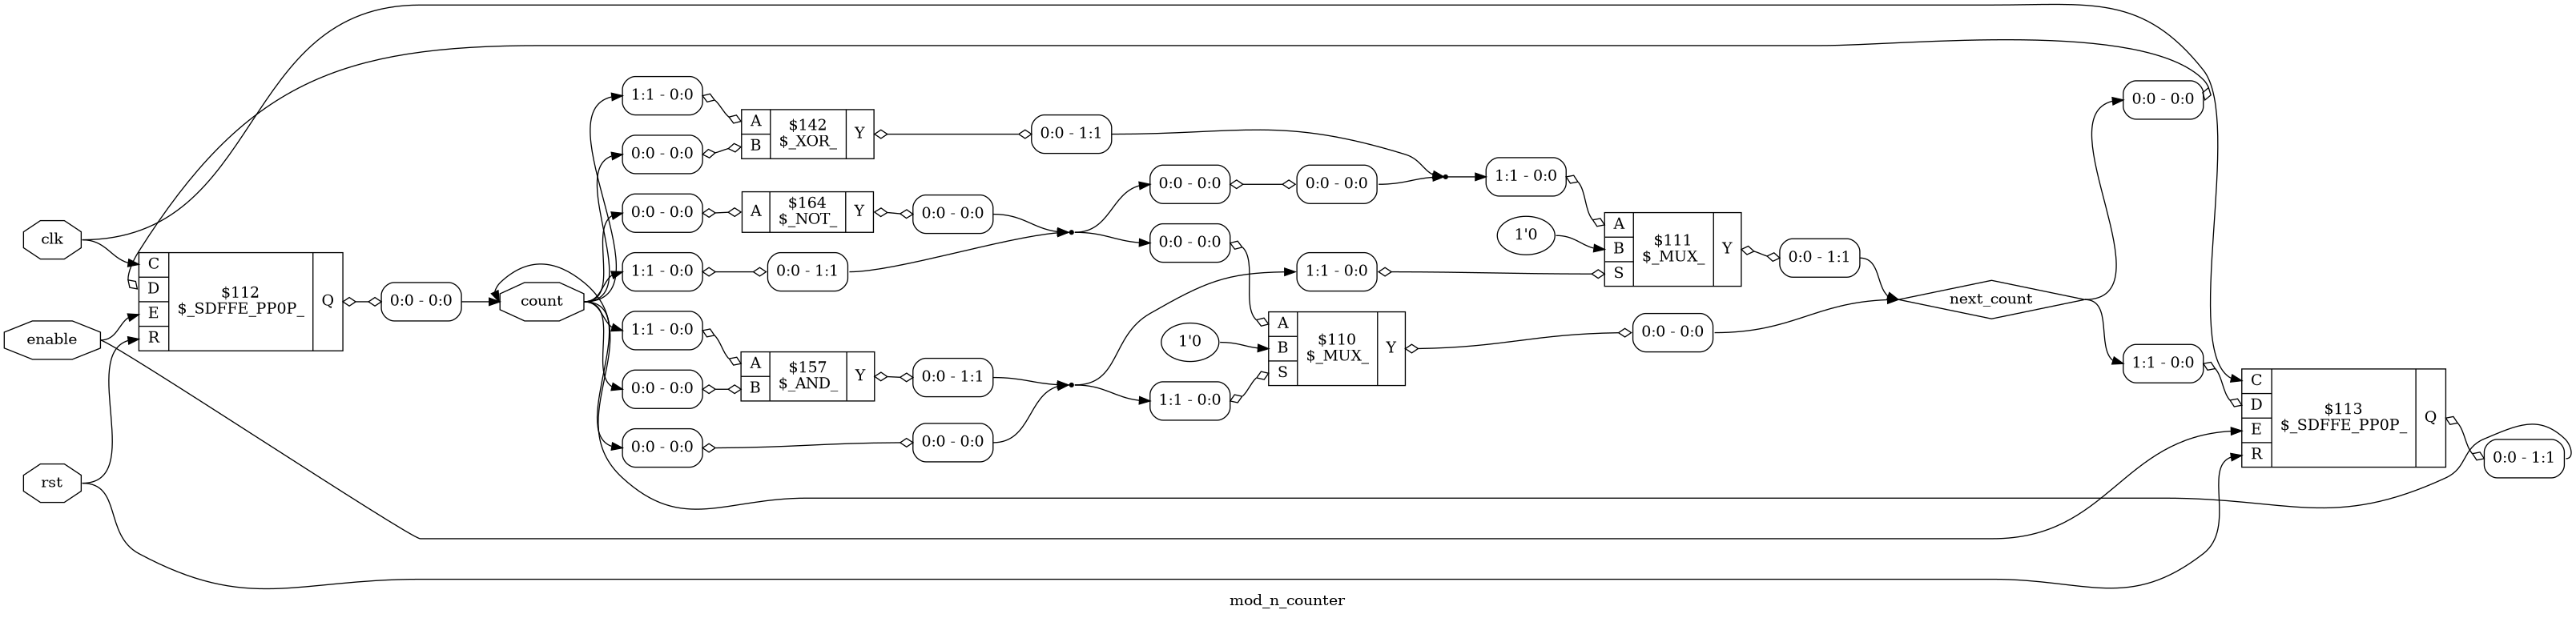
\includegraphics[width=\linewidth]{Images/abc.png}
  \caption{Abc diagram produced by yosys.}
  \label{fig:procyosys}
\end{figure}

\subsection{Report 20}
No extra features were added. Time was focused on testing and debugging. 

\subsection{Report 21}
Basic clocking, rising edge detection and counting is the ideal use case for 
digital logic on an FPGA. However, 

\end{document}